\documentclass[oneside,12pt]{Classes/aesm_edspia}
\usepackage{minitoc}
\usepackage[utf8]{inputenc}
\usepackage[english,french]{babel}
\usepackage[T1]{fontenc}
\usepackage{amsmath}
\usepackage{lmodern}%font modern
\usepackage[bottom]{footmisc}
\rmfamily
\usepackage[section]{placeins}

\DeclareFontShape{T1}{lmr}{bx}{sc}{<->ssub * cmr/bx/sc}{} 
\usepackage{lettrine}
\usepackage{tabularx}
\usepackage{epsfig, floatflt, amssymb} 
\usepackage{moreverb} %% pour le verbatim en boite
\usepackage{cases}%equations en systemes numérotés - soluce possible package : CASES
\usepackage{multirow} %% pour regrouper un texte sur plusieurs lignes dans une table
\usepackage{url} %% pour citer les url par \url
\usepackage[all]{xy} %% pour la barre au dessus des symboles
\usepackage{textcomp} %% pour le symbol pour mille par \textperthousand et degrés par \degres
\usepackage[right]{eurosym}
\usepackage{setspace} %interligne simple, double etc...
\usepackage{Classes/eurosans} %%pour le symbole \euro
\usepackage{epic,eepic}
\usepackage{soul}
\usepackage[nottoc]{tocbibind} % tables des figures, des matieres et autres dans la TOC

\usepackage[titles]{tocloft}
\usepackage{fancybox}
\usepackage[leftcaption]{sidecap}
\usepackage[labelsep=endash, textfont={footnotesize, singlespacing}, margin=10pt, format=plain, labelfont=bf]{caption}
\usepackage[Conny]{Classes/fncychap} %en tete chapitrage}
\newcommand{\ie}{c.-\`a-d.~}
\hbadness=10000% pb d'overfull box réglé
\hfuzz=50pt
\def\underscore{\char`\_}
\makeatletter
\renewcommand{\thesection}{\arabic {section}}
\renewcommand{\SC@figure@vpos}{c}% centrer verticalement le caption avec le package sidecap...
\renewcommand{\fnum@figure}{\small\textbf{Figure~\thefigure}}
\renewcommand{\fnum@table}{\small\textbf{Tableau~\thetable}}
 \renewcommand*\l@figure{\@dottedtocline{1}{1em}{3.2em}}
 \renewcommand*\l@table{\@dottedtocline{1}{1em}{3.2em}}




\makeatother
\usepackage{subfig}
\def\thechapter{\Roman{chapter}}

%\usepackage[framed,numbered,autolinebreaks,useliterate]{Classes/mcode}


%%% Listings

\usepackage{listings}
\lstloadlanguages{xml, java}
	
	 \usepackage{listings}
  \usepackage{courier}
 \lstset{
         basicstyle=\footnotesize\ttfamily, 
         %numbers=left,               
         numberstyle=\tiny,          
         %stepnumber=2,               
         numbersep=5pt,              
         tabsize=2,                  
         extendedchars=true,         
         breaklines=true,            
         keywordstyle=\color[rgb]{0.43,0,0}\textbf,
    		frame=b,
         commentstyle=\color[rgb]{0.51,0.51,0.51} \textit ,
         stringstyle=\ttfamily  \color[rgb]{0,0.44,0} ,
         showspaces=false,           
         showtabs=false,             
         xleftmargin=17pt,
         framexleftmargin=17pt,
         framexrightmargin=5pt,
         framexbottommargin=4pt,
         %backgroundcolor=\color{lightgray},
         showstringspaces=false            
 }
 
 \usepackage{caption}
\DeclareCaptionFont{white}{\color{white}}
\DeclareCaptionFont{red}{\color{red}}
\DeclareCaptionFont{black}{\color{black}}
\DeclareCaptionFormat{listing}{\colorbox[cmyk]{0.43, 0.35, 0.35,0.01}{\parbox{\textwidth}{\hspace{15pt}#1#2#3}}}
\captionsetup[lstlisting]{format=listing,labelfont=black,textfont=white, singlelinecheck=false, margin=0pt, font={bf,footnotesize}}

%%%%%%%%%%%%%%%%%%%%%%%%%%%%%%%%%%%%%%%%%%%
\begin{document}
%%%%%%%%%%%%%%%%%%%%%%%%%%%%%%%%%%%%%%%%%%%
\renewcommand\figurename{\small\textbf{Figure}} 

\addtocounter{page}{-1}%pour revenir � 0

%%%%%%%%%%%%%%%%%%%%%%%%%%%%%%%%%%%%%%%%%%%
\makethese %% crée la couverture.



\newpage\thispagestyle{empty}
\makesecondthese

\newpage\thispagestyle{empty}
\null

\newpage\thispagestyle{empty}
\frontmatter %num�rotation en iii

\chapter*{Dedicaces}
%===================================================================
\begin{spacing}{1.5}
{\fontfamily{cmr}\selectfont
\noindent
\itshape{
\Large{À \textbf{ma très chère mère}}
}\\
\noindent
\textit{
\large{Si Dieu a mis le paradis sous les pieds des mères, ce n’est pas pour rien. Autant de phrases aussi expressives soient-elles ne sauraient montrer le degré d’amour et d’affection que j’éprouve pour toi. Tu m’as comblé avec ta tendresse et affection tout au long de mon parcours. En ce jour mémorable, reçoit ce travail en signe de ma vive reconnaissance et ma profonde estime. Puisse le tout puissant te donner santé, bonheur et longue vie afin que je puisse te combler à mon tour.}}\\

\noindent
\itshape{
\Large{À \textbf{mon très cher père}}
}\\
\noindent
\textit{
\large{Autant de phrases et d’expressions aussi éloquentes soient-elle ne sauraient exprimer ma gratitude et ma reconnaissance. Tu as su m’inculquer le sens de la responsabilité, de l’optimisme et de la confiance en soi face aux difficultés de la vie. Je te dois ce que je suis aujourd’hui et ce que je serai demain et je ferai toujours de mon mieux pour rester ta fierté et ne jamais te décevoir. Que Dieu le tout puissant t’accorde santé, bonheur et te protège de tout mal.}}\\

\noindent
\itshape{
\Large{À \textbf{mes belles soeurs}}
}\\
\noindent
\textit{
\large{Ce travail est un témoignage aux plus belles soeurs du monde, qui n'ont plus cessé de me supporter.}}\\

\noindent
\itshape{
\Large{À tous \textbf{mes professeurs à l’INSAT}}
}\\
\noindent
\textit{
\large{Je dédie ce modeste travail à mes professeurs qui m'ont appris des leçons et des valeurs précieux dans ma vie. Je profite de cette occasion pour leur exprimer ma profonde gratitude et couronnement de leur assistance.}}

}
\end{spacing}
\pagestyle{fancy}
\fancyhf{}
\fancyhead[R]{Dedicaces}
\fancyfoot[R]{\thepage}
\renewcommand{\headrulewidth}{0.5pt}
\renewcommand{\footrulewidth}{0pt}
\newcommand{\limitpages}[1]

\chapter*{Remerciements}
%===================================================================
\vspace{2cm}

L’élaboration de ce rapport n’aurait été possible sans l’intervention de certaines personnes. Qu’elles trouvent ici l’expression de nos plus sincères remerciements pour leurs précieux conseils.\\

Nous nous adressons en premier lieu aux membres de l’honorable jury que nous remercions d’avoir accepté d’examiner ce rapport en espérant qu’ils y trouvent les qualités de clarté et de motivation qu’ils attendent.\\

Nous adressons également nos vifs remerciements à notre encadrante, Mme. Ghada GASMI, Enseignante universitaire, pour ses conseils, son assistance et son soutien tout au long de la période de stage.\\

Nous tiendrons à remercier vivement notre tuteur professionnel, Mme. Valérie NOYER, Release manager, pour son accueil, le temps passé ensemble et le partage de son expertise au quotidien. Grâce aussi à sa confiance nous avons pu nous accomplir totalement dans nos missions. Elle fut d'une aide précieuse dans les moments les plus délicats.\\

Nos remerciements s’étendent également à Mr Nicolas DERYCKE, notre directeur technique, pour ses conseils avisés et son encouragement, ainsi qu'à toute l’équipe de Konvergence Business \& Technologies qui a essayé de créer une ambiance favorable au bon déroulement de ce stage.\\

Nos profonds remerciements vont également aux amis anciens Insatiens qui travaillent à Konvergence pour leurs supports et conseilles tout au long de la durée de notre stage.\\

Enfin, nous tenons à remercier toutes les personnes qui ont participé de près ou de loin à la réalisation de ce travail.

\pagestyle{fancy}
\fancyhf{}
\fancyhead[R]{Glossaire}
\fancyfoot[R]{\thepage}
\renewcommand{\headrulewidth}{0.5pt}
\renewcommand{\footrulewidth}{0pt}
\newcommand{\limitpages}[1]

\chapter*{Glossaire}
\addcontentsline{toc}{chapter}{Glossaire}

%===================================================================

\textbf{AMQP} : Advanced Message Queuing Protocol\\

\textbf{API} : Application Programming Interface\\

\textbf{BAM}: Business Activity Monitoring\\

\textbf{BI}: Business Intelligence\\

\textbf{CLI} : Command Line Interface\\

\textbf{CSV} : Comma-Separated Values\\

\textbf{DB} : DataBase\\

\textbf{DevOps} : Development and Operations\\

\textbf{Dev} : Development\\

\textbf{EPM} : Enterprise Performance Management\\

\textbf{ETL} : Extract Transform Load \\

\textbf{EaC} : Everything as Code\\

\textbf{GRC} : Governance, Risk \& Compliance\\

\textbf{IASB} : International Accounting Standards Board\\

\textbf{IFRS16} : International Financial Reporting Standards 2016\\

\textbf{IHM} : Interface Homme Machine\\


\textbf{IaC} : Infrastructure as Code\\

\textbf{JEXL} : Java Extended Expression Language\\

\textbf{JFR} : Java Flight Recorder\\

\textbf{JMC} : Java Mission Control\\

\textbf{JMX} : Java Management eXtensions\\

\textbf{MQTT} : Message Queuing Telemetry Transport\\

\textbf{Ops} : Operations\\

\textbf{PDF} : Portable Document Format\\

\textbf{POM} : Project Object Model\\

\textbf{PaC} : Pipeline as Code\\

\textbf{QA} : Quality Assurance\\

\textbf{RD} : Research and Development\\

\textbf{REST} : Representational State Transfer\\

\textbf{SGBDR} : Système de Gestion de Base de Données Relationelles\\

\textbf{SQL} : Structured Query Language\\

\textbf{SSH} : Secure Shell\\

\textbf{SVN} : Subversion\\

\textbf{SaaS} : Software as a Service\\

\textbf{VCS} : Version Control System\\

\textbf{WebDav} : Web-based Distributed Authoring and Versioning\\

\textbf{XML} : eXtensible Markup Language\\

\textbf{YML} : Yet another Markup Language\\
\pagestyle{fancy}
\fancyhf{}
\fancyhead[R]{Glossaire}
\fancyfoot[R]{\thepage}
\renewcommand{\headrulewidth}{0.5pt}
\renewcommand{\footrulewidth}{0pt}
\newcommand{\limitpages}[1]


%%%%%%%% TOC

%profondeur dans la table des mati�res et de la num�rotation des sections

\setcounter{secnumdepth}{3}
\setcounter{tocdepth}{3}


\renewcommand{\contentsname}%
    {Table des Matières}%

%%%%minitoc
\dominitoc % g�n�re la minitoc
\nomtcrule % supprime les lignes horizontales de la minitoc
\renewcommand{\mtctitle}{Plan} % Modifie le titre de la minitoc

%%%%
\tableofcontents

\renewcommand{\headrulewidth}{0.5pt}
\renewcommand{\footrulewidth}{0pt}
\fancyhead[R]{Table des Matières}


%%%%%%%% Figures

\makeatletter
%\renewcommand{a\thefigure}{\@arabic\c@figure}
\@addtoreset{figure}{chapter}
\makeatother

\renewcommand{\headrulewidth}{0.5pt}
\renewcommand{\footrulewidth}{0pt}
\renewcommand\listfigurename{Liste des Figures}
\listoffigures \mtcaddchapter 

\fancyhead[R]{Liste des Figures}
\newpage


%%%%%%%% Tableaux

\makeatletter

\renewcommand{\headrulewidth}{0.5pt}
\renewcommand{\footrulewidth}{0pt}
\renewcommand\listtablename{Liste des Tableaux}

\listoftables  \mtcaddchapter 

\fancyhead[R]{Liste des Tableaux}

%%%%%%%%%%%%%%%%%%%%%%%%%%%%%%%%%%%
%\fancyhead[R]{R�sum�s}

\chapter*{Résumé}
\addcontentsline{toc}{chapter}{Résumé}
%===================================================================

Ce rapport couvre les phases de conception, développement, test et mise en place des chaines d'intégration et livraison continues, et les travaux d'automatisation effectués au sein de la société Konvergence. Nous expliquerons aussi les étapes de chaque phase en justifiant les choix technologiques ainsi que les paradigmes utilisés.\\ 

Nous allons commencer par mettre en place trois chaines d'intégration et livraison continues, pour les différentes versions de l'application IFRS16, un produit principal basé sur la plateforme Shuttle, qu'on découvrira dans le deuxième chapitre. Ces chaines permettent la construction de l'application IFRS16, le test et le retour rapide des éventuelles anomalies.\\

La deuxième partie du stage consiste à concevoir un mécanisme automatique de lancement des tests de performance pour la plateforme Shuttle et de reporting des résultats. Étant donné les grosses volumétries gérées par les applications Shuttle, la stabilité des temps de réponse est une contrainte très importante.\\

Ces projets ont nécessité tout d’abord une familiarisation avec la solution Shuttle, une solution logicielle unifiée et collaborative dédiée au pilotage de la décision dans les domaines de la performance financière et opérationnelle et éditée et maintenue par Konvergence business \& Technologies, ainsi que les outils utilisés pour le déploiement et test de la plateforme. Une étude des concepts de base de l’intégration continue, les tests automatiques et la livraison continue s'impose pour bien acquérir les connaissances nécessaires afin d'implémenter un système adapté à un produit complexe tel que Shuttle.\\

\chapter*{Abstract}
\addcontentsline{toc}{chapter}{Abstract}
%===================================================================

This report covers the design, development, testing and implementation phases of the continuous integration and delivery pipelines, and the automation tasks done within Konvergence. We will also explain the steps of each phase, emphasizing the technological choices and adopted paradigms.\\

We'll start by setting up three continuous integration and delivery pipelines for different versions of the IFRS16 application, a major product based on the Shuttle. These pipelines allow the build of the IFRS16 application, the test and rapid feedback the eventual problems.\\

The second part of this internship consists in designing an automatic mechanism for running the performance tests for the Shuttle platform and reporting the results. Given the big volumes treated by Shuttle applications, the stability of response time is a very important constraint.\\

These projects required first of all a familiarization with the Shuttle solution, a unified and collaborative software dedicated to decision management in the areas of financial and operational performance and edited and maintained by Konvergence, as well as the tools used for the deployment and testing of the platform. A study of the basic concepts of continuous integration, automatic testing and continuous delivery is necessary to acquire the necessary knowledge to implement complex workflows for a tool such as the Shuttle.\\


%%%%%%%%%%%%%%%%%%%%%%%%%%%%%%%%%%%

                       
\mainmatter %num�ros arabes
\pagestyle{fancy}
\fancyhead[R]{Introduction Générale}
\chapter*{Introduction Générale}
\addcontentsline{toc}{chapter}{Introduction Générale}
\begin{spacing}{1.2}
%==================================================================================================%

L’origine du terme “Intégration Continue” revient à l’américain Grady Booch\cite{gardBooch}, co-développeur du langage de modélisation UML, qui a introduit le terme ‘Continuous Integration'\cite{continuousIntegration} dans sa méthode de développement de logiciels orientés objets. En revanche, Booch n’a pas préconisé le terme. L’intégration continue revient dans le monde de développement logiciel en mai 2006 avec le Britannique Martin Fowler, un des gros acteurs dans le domaine de conception de logiciels d’entreprise. 
Fowler a expliqué et mit l’emphase sur le concept dans sa publication\cite{martinFowler}.\\

“Continuous Integration is a software development practice where members of a team integrate their work frequently, usually each person integrates at least daily - leading to multiple integrations per day. Each integration is verified by an automated build (including test) to detect integration errors as quickly as possible. Many teams find that this approach leads to significantly reduced integration problems and allows a team to develop cohesive software more rapidly.” [Continuous Integration, Martin Fowler, 1 Mai 2006]\\

Offrant une large gamme d'applications d'aide à la décision dans différents domaines, Konvergence Business \& Technologies s'engage pour satisfaire ses clients, avec une suite logicielle de qualité, testée et livrée dans les temps, avec une ouverture pour les retours d'expériences et le signalement des disfonctionnements (bugs).\\

C'est dans cette perspective, et pour assurer un processus d'intégration, de test et de livraison continues de ses applications, le département recherche et développement de la boite a entamé la mise au point de la pratique DevOps qui part des besoins, bugs, et retours clientes, à la livraison des applications.\\

Dans ce que suit, nous présentons la structure de notre rapport:
\begin{itemize}
\setlength\itemsep{0em}
\item Le premier chapitre intitulé "Cadre du projet" dans lequel, nous présenterons la société d’accueil, la méthodologie de travail et quelques concepts de base.
\item Le deuxième chapitre "IFRS16 CI/CD Pipelines" présentera les chaines d'intégration continue et l'automatisation de tests de l'application IFRS16.
\item Le troisième chapitre " ench Tests Pipeline" présentera la conception et la mise en place du pipeline de Bench Tests, les tests de performance de la plateforme Shuttle. 
\end{itemize}

Nous finissons notre rapport par une conclusion générale dans laquelle nous discuterons les différents travaux réalisés et les perspectives.
\end{spacing}
\fancyhf{}
\fancyhead[R]{Introduction Générale}
\fancyfoot[R]{\thepage}
\renewcommand{\headrulewidth}{0.5pt}
\renewcommand{\footrulewidth}{0pt}



\setcounter{mtc}{5} %indique le num�ro r�el du chapitre, pour la mini table des mati�res
\chapter{Cadre du projet}
\minitoc %insert la minitoc
\graphicspath{{Chapitre1/figures/}}
%==============================================================================
\pagestyle{fancy}
\fancyhf{}
\fancyhead[R]{\bfseries\rightmark}
\fancyfoot[R]{\thepage}
\renewcommand{\headrulewidth}{0.5pt}
\renewcommand{\footrulewidth}{0pt}
\renewcommand{\chaptermark}[1]{\markboth{\MakeUppercase{\chaptername~\thechapter. #1 }}{}}
\renewcommand{\sectionmark}[1]{\markright{\thechapter.\thesection~ #1}}

\begin{spacing}{1.2}
%==============================================================================
\section*{Introduction}
Ce premier chapitre a pour objectif de situer le projet dans son cadre général. Nous présenterons donc l’organisme d’accueil, son historique et ses secteurs d'activité. Nous enchaînerons sur les problématiques et les solutions proposées, la méthodologie de travail adoptée et nous achèverons par une présentation de quelques concepts de base et étude de l’existant.
\vspace{-3mm}
\section{Présentation de l'organisme d’accueil: Konvergence B\&T}
\subsection{Présentation générale}
Basée à Paris, Konvergence a été fondée en janvier 1987. Société par actions simplifiées, à associé unique, elle compte 65 salariés. L'effectif est divisé en trois départements majeurs: R\&D, Services et Consulting. Grâce à son personnel très actif, l’entreprise a réussi à imposer sa place parmi les leaders mondiaux de son marché avec un chiffre d'affaires de 31 000,00 € pour l'année 2006 et à se développer également au niveau international avec l’ouverture d’une filiale aux Etats-Unis et en Tunisie. Le total de son bilan a augmenté de 99,00 \% entre 2005 et 2006.\\

À l'origine, intégrateur de solutions de mesure de la performance financière des solutions Oracle Hyperion, Konvergence a conçu initialement le logiciel Shuttle comme un Add-On\footnote{extension à un autre logiciel} renforçant la plateforme Oracle Hyperion Essbase. Au fil du temps, Shuttle est devenu une plateforme à part entière\cite{shuttle}, concurrente de celle d'Oracle. De ce fait, Konvergence a décidé de faire une spin-off et rendre le Shuttle indépendant et quitter l'activité d'intégration des solutions Hyperion Essbase. 
Aujourd'hui, la boite est spécialisée dans l’édition de logiciels applicatifs et l'intégration des ses propres solutions BI/EPM.

\subsection{Secteurs d'activité}
Konvergence est l’éditeur de la solution Shuttle, une solution dédiée au pilotage de la décision dans les domaines de la performance financière et opérationnelle, de la gestion des risques et de la gouvernance. Elle intègre au sein d’une seule plateforme des fonctionnalités de collecte de données, de gestion de bases de données, de restitution, d'aide à la décision, de Disclosure Management et de Reporting  [annexe A.1]. Cette solution est déployée à l’international et rencontre un succès croissant auprès de ses clients. Elle offre une plateforme évolutive avec une efficacité opérationnelle permettant de créer dynamiquement des applications intégrées d'EPM, de BI, de BAM et de GRC [annexe A.1]. 
La figure I.1 montre les clients de Konvergence par domaine d'application.
\begin{figure}[H]\centering 
	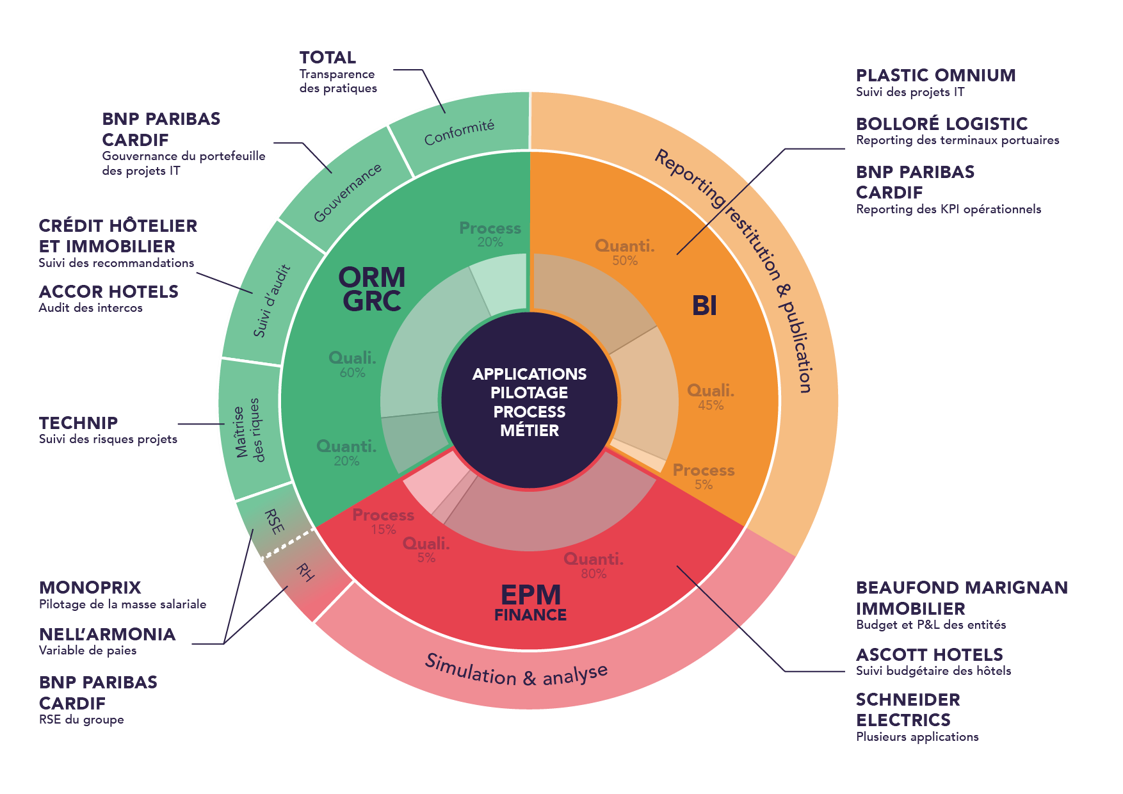
\includegraphics[scale=0.5]{solutions}
	\caption{Clients Shuttle par domaine}\cite{intern}
	\label{fig:fig2}
\end{figure}

%La figure A.1 présente l'architecture applicative de la solution Shuttle.
\vspace{-3mm}
\section{Présentation des projets}
\subsection{Intégration continue et tests automatiques IFRS16}
\subsubsection{Contexte et problématiques}

Les normes IFRS ont pour objectif d’harmoniser la présentation des états financiers des entreprises.
L'IASB a publié le 13 janvier 2016 la norme IFRS 16\cite{ifrs16}. 
Très brièvement, IFRS 16 est un standard de finance qui désormais impose la comptabilisation au bilan du preneur de tous les contrats de location.
Nombreuses entreprises, indépendamment de leur secteur d’activité, font le choix d’intégrer dans leurs systèmes d’information des outils informatiques permettant la mise en œuvre de cette norme.

Conciente de cet enjeu, Konvergence édite une application nommée "K-IFRS16", qui offre la facilité de gestion et de suivi d’un volume important de contrats de locations établis conformément à la norme IFRS 16. Cette application est basée sur les solutions propriétaires de l’entreprise : la plateforme Shuttle. 

Konvergence a mis en oeuvre une équipe dédiée à l'édition de l'outil K-IFRS16. Des consultants, fonctionnels, experts comptables, des développeurs et des testeurs ont pour mission de développer et assurer la livraison d'un produit de qualité à leur clients.

Toutefois, les tests de cet outil sont faites manuellement, donnant plus de chance à l'erreur humaine et prennant beaucoup de temps et effort.

Le processus de développement et test de l'application est comme suit : 
\begin{itemize}
\setlength\itemsep{0em}
    \item Un consultant fonctionnel demande à l'équipe de développeurs d'ajouter une fonctionnalité en les expliquant le besoin.
    \item Les développeurs implémentent le besoin, rajoutent des tests unitaires et livrent la nouvelle application aux testeurs.
    \item Les testeurs font appelles aux consultants pour demander les scénarios de tests possibles et les résultats attendus.
    \item Les consultants décrivent les scénarios et fournissent les résultats attendus sous forme de fichiers CSV.
    \item Les testeurs, après avoir exécuté les scénarios à la main, comparent les résultats case par case. En cas d'erreur, ils appellent les fonctionnels et les développeurs pour investiguer les anomalies.
\end{itemize}
De plus, la livraison de l'application était manuelle. Un processus long demeurant de plus en plus difficile, avec la multitude de version et configuration.
\subsubsection{Solution proposée : IFRS16 CI/CD Pipelines}
Dans ce cadre, nous avons mis en place trois chaines d'intégration et livraison continues pour les différentes versions de l'application K-IFRS16. Partant de l'outil de gestion de code source, un pipeline IFRS16, construit le projet, exécute les tests unitaires, déploie les artefacts, prépare un environnement Cloud de tests et exécute les différents scénarios de tests de non-regréssion. Nous verrons plus en détails ces pipelines dans le chapitre qui suit. 
\subsection{Automatisation du processus de Benchmark Tests}
\subsubsection{Contexte et problématiques}
Shuttle est un outil de BI/EPM puissant et très flexible\cite{intern}. Il offre la compatibilité avec une large gamme de bases de données relationnelles et tourne sur les trois systèmes d'exploitation les plus utilisés: Windows, Mac et Linux. Étant données les préférences et les spécificités de chaque client, le bon fonctionnement, la non-régression, les performances et la haute disponibilité de la plateforme sont des contraintes très importantes. 
Pour assurer ces dernières, des tests de performance, "Benchmark Tests", sont nécessaires sur les différents environnements offerts. 
Le processus de Benchmark tests était manuel. L'ingénieur QA commence par la création et le déploiement de l'environnement, ensuite il lance les tests, puis il enregistre les résultats sous forme de fichiers CSV pour les synthétiser enfin dans une feuille Excel. Cette méthode est assez lente et nécessite beaucoup de concentration. De plus, le reporting étant statique, ceci rend l'investigation des résultats très difficile. 
C'est dans ce contexte que le projet de "Bench Tests Pipeline" a été nécessaire.
\subsubsection{Solution proposée : Bench Tests Pipeline}
Nous allons mettre en place un mécanisme automatique de construction d'environnement Shuttle, de lancement des tests de performance et de reporting des résultats. Cette solution offre la flexibilité dans les choix des services et bases de données à déployer dans l'environnement cloud, la durée des tests et différents indicateurs et graphiques pour le reporting.
\section{Méthodologie de travail : Scrum}
\subsection{Méthodologie agile}
En février 2001, aux Etats Unis, 17 spécialistes du développement logiciel se sont réunis pour débattre du thème unificateur de leurs méthodes respectives, dites méthodes agiles. De cette réunion a émergé le Manifeste Agile considéré comme la définition canonique du développement Agile et de ses principes sous-jacents. 

Durant notre projet, nous avons intégré principalement l'équipe R\&D qui applique l'agilité depuis 3 ans.
Constituée de 12 personnes dont un Release Manager, un ingénieur DevOps, huit développeurs, un architecte et un Product Owner, nous avons assuré la partie DevOps au sein de cette équipe. Nous avons fait le relais entre les différentes équipes de la boite en travaillant également à la fois avec l'équipe de développement de la plateforme, l'équipe Apps qui développent les applications en utilisant le Shuttle, l'équipe Ops et l'équipe IT. Le but était d'éliminer les silos et permettre une meilleure intéraction dans la boite. Nous avons bien entendu adopté une méthode agile pour le pilotage de nos projets, c'est la méthode Scrum.

Cette méthodologie offre une meilleure adaptabilité, visibilité et gestion des risques. Elle se caractérise par un modèle de développement itératif, où les exigences et les solutions évoluent grâce à la collaboration entre des équipes interfonctionnelles, un processus de gestion de projet qui encourage une inspection et une adaptation fréquentes, l'auto-organisation et la responsabilisation, un ensemble de valeurs et de bonnes pratiques et une approche métier alignant le développement sur les besoins des clients et les objectifs de l'entreprise. Elle fait référence à tout processus de développement aligné sur les concepts du Manifeste Agile [annexe B]\cite{manifesto}.
\subsection{Scrum}
Scrum, un cadre de processus léger pour le développement agile, est le plus souvent utilisé pour la gestion des projets complexes. Il se distingue des autres processus agiles par des concepts et des pratiques spécifiques, divisés en trois catégories : Rôles, Artefacts et Boîtes de temps. Cette méthodologie a comme objectif d’augmenter la productivité et la qualité des livrables et de réduire le délai d'obtention des avantages par rapport aux processus "cascade" classiques. Elle permet aux équipes de s'adapter facilement à l’évolution rapide des exigences et de répondre aux changements d’objectifs des métiers qui sont en constante évolution.
La construction du produit se fait en plusieurs itérations d'une durée de 2 à 4 semaines nommées "Sprint". Durant chacune de ces itérations, une partie du produit nommée "Incrément" est réalisée en se basant sur ce qui précède et est livrée à la fin du sprint. La figure I.2 explique le déroulement du processus Scrum.
\begin{figure}[!ht]\centering
\includegraphics[scale=0.22]{"scrum".png}
\caption{Cycle de vie d'un processus Scrum \cite{scrum}}
\label{fig:fig1}
\end{figure}
\FloatBarrier
\textbf{Rôles:}
\begin{itemize}
\setlength\itemsep{0em}
    \item[--] Scrum Master : Le gardien du processus. Responsable du bon déroulement du processus, de l'élimination des obstacles et de l'organisation des réunions critiques.
    \item[--] Product Owner : Le gardien des exigences. La « source unique de vérité » en ce qui concerne les exigences et l'ordre de mise en œuvre planifié. C'est l'interface entre l'entreprise, les clients et leurs besoins liés aux produits d'un côté, et l'équipe de l'autre.
    \item[--] Equipe Scrum : Une équipe auto-organisée et interfonctionnelle, comptant idéalement entre cinq et neuf personnes, qui effectue le travail de développement et de test. Elle a également le pouvoir de prendre des décisions sur la façon d'effectuer le travail.
\end{itemize}

\textbf{Product Backlog : }
Une liste ordonnée de tout ce qui doit être fait, les exigences fonctionnelles et non fonctionnelles, sous forme de user story qui remplace les artefacts de spécification des exigences traditionnelles.

\textbf{Réunions : }
\begin{itemize}
\setlength\itemsep{0em}
\item[--] Planification du sprint : Se déroule au début de chaque sprint, dans le but de mettre en place une liste d'éléments prioritaires du Product Backlog à réaliser au cours du sprint.   
\item[--] Revue de sprint: Présenter, à la fin du sprint, le travail accompli par l’équipe lors du dernier sprint.
\item[--] Rétrospective de sprint : A pour objectif de découvrir ce qui a bien fonctionné et ce qui n'a pas fonctionné lors du dernier sprint et comment s'améliorer.
\item[--] Mêlée quotidienne : Se tient tous les jours et se fait debout pour que la réunion soit courte et précise. Elle permet aux membres de l’équipe de s'informer mutuellement.
\end{itemize}
\subsection{Équipe et rôles}
Durant notre stage, nous avons intégré l’équipe R\&D chez Konvergence. L’équipe compte 12 personnes. Elle se décompose en un ensemble des sous-équipes interfonctionnelles qui collaborent entre elles. Nous allons travailler avec toutes ces équipes, ainsi que d'autres, en faisant le relais entre les Devs, l'IT et l'Ops. Nous allons collaborer notamment avec la Release Manager pour assurer les tests automatiques, l'intégration et la livraison continues.
\begin{table}[ht]
	\centering
	\caption{Rôle et membres}
	\footnotesize
	\begin{tabularx}{\textwidth}{|X|X|}
          \hline
          {\textbf{Rôle}}
          & 
          {\textbf{Membres}} 
          \\
          \hline
          Release Manager & Mme. Valérie NOYER \\    \hline
          Scrum Master & Mr. Hamza NOURI \\          \hline
          Product Owner & Mr. Nicolas DERYCKE \\          \hline
          Operations & Mr. Olivier ROCHON \\          \hline
          IT Infrastructure  & Mr. Paul LECLERC \\          \hline
          Testeurs & Mr. Nader KASRI \\          \hline
          Stagiaire CI/CD DevOps & Rafik BAHRI \\          \hline
          Dev & Les développeurs \\          \hline
        \end{tabularx}
	\label{tab:exple}
\end{table}
\FloatBarrier
Nous avons divisé nos travaux en Sprints par sujet. La figure I.3 explique le déroulement de notre stage. 
\begin{figure}[H]\centering
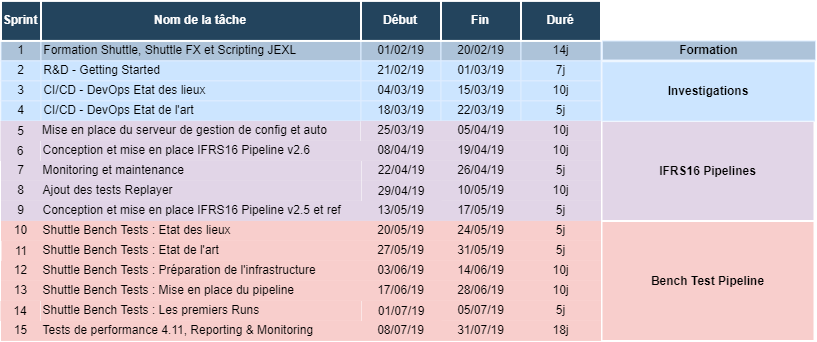
\includegraphics[scale=0.5]{Chapitre2/figures/gant.png}
\caption{La liste des sprints}
\label{fig:fig1}
\end{figure}
\FloatBarrier
Nous allons aborder, dans le paragraphe qui suit, quelques concepts de base ainsi que l'état des lieux que nous avons fait.
\section{Concepts de base et étude de l’existant}
\subsection{CI/CD et DevOps}
\textbf{CI (Continuous Integration)} : La pratique utilisée en Génie Logiciel permettant d'intégrer plusieurs fois pendant la journée les changements effectués sur le code du projet, et ceci d'une manière automatique qui déclenche un build et les tests, afin de détecter les erreurs et les régressions au plus tôt possible. 

\textbf{CD (Continuous Delivery/Deployment)} : L'acronyme CD peut etre utilisé pour décrire l'un des termes : 
\begin{itemize}
    \item Continuous Delivery : La livraison continue est l'approche dans laquelle les équipes produisent des logiciels dans des cycles courts, ce qui permet de le mettre à disposition à n’importe quel moment. Le but est de construire, tester et diffuser un logiciel plus rapidement.
    \item Continuous Deploiment : Le déploiement continué est la stratégie de développement où toute validation de code qui réussit le cycle de build et test automatiques est transférée dans l'environnement de production, propulsant ainsi les modifications vers les utilisateurs finaux du logiciel.
\end{itemize}
\begin{figure}[H]\centering
\includegraphics[scale=0.3]{"devops-cycle-without-deployement".png}
\caption{Process d'intégration et livraison continue existant du Shuttle}
\label{fig:fig2}
\end{figure}

\textbf{DevOps (Development \& Operations)} : DevOps est un ensemble de pratiques qui met l'accent sur la collaboration et la communication entre les développeurs de logiciels et les professionnels des opérations informatiques, en automatisant le processus de livraison de logiciels et les changements d'infrastructure.

\begin{figure}[H]\centering
\includegraphics[scale=0.25]{"devops".png}
\caption{Cycle DevOps}
\label{fig:fig3}
\end{figure}
Le cycle de DevOps se décompose comme suit : 
\begin{enumerate}
\setlength\itemsep{0em}
      \item Plan : la planification des différentes taches, tickets et autres jalons
      \item Create : la concrétisation des taches planifiées
      \item Verify : le test et l'acceptance des développements effectués
      \item Package : la construction des artefacts prêts à la livraison
      \item Release : la livraison des artefacts après tests
      \item Configure : la configuration et le déploiement des produits
      \item Monitor : la surveillance des produits ainsi déployés
\end{enumerate}

\subsection{Étude de l’existant}
\textbf{La palteforme} : Shuttle est une solution logicielle unifiée et collaborative, dédiée au pilotage de la décision Son modèle collaboratif est renforcé par sa capacité à gérer tout processus et à aider l'entreprise à progresser vers l'excellence opérationnelle. La figure I.4 décrit l'architecture technique de la solution Shuttle.
\begin{figure}[H]\centering
\includegraphics[scale=0.4]{"shuttle arch app".PNG}
\caption{Architecture technique de la solution Shuttle}
\label{fig:fig4}
\end{figure}
\FloatBarrier
Elle est composée du :
\begin{itemize}
    \setlength\itemsep{0em}
    \item[--] Référentiel : constitué des métadonnées dont l’application a besoin pour fonctionner.
    \item[--] Des règles de calcul : Shuttle possède  un moteur de calcul afin de centraliser ces règles.
    \item[--] D’un processus métier digitalisé à l’aide de Shuttle.
    \item[--] D’un dispositif de sécurité d’accès aux métadonnées, aux données et aux objets applicatifs.
    \item[--] D’un moteur de stockage de données propriétaire ShuttleDB : une technologie unique hybride, qui combine à la fois les caractéristiques OLAP [annexe A.3] et OLTP [annexe A.4].
    \item[--] D’applications client qui offrent des interfaces permettant de collecter de l’information auprès de l’utilisateur et des rapports qui présentent le résultat de la restitution de ces données.
\end{itemize}

\FloatBarrier
\textbf {Le serveur} : C'est la partie Backend de la plateforme. Le serveur Shuttle est l'outil permettant la conception des applications, la modélisation des données dans des cubes multi-dimesionels ainsi que la construction des IHM. Il permet également aux administrateurs de gérer les droits d'accès, la sécurité des applications et des données. 

\textbf {Le client} : Shuttle FX est le nom du client de la plateforme Shuttle. C'est une application Desktop basée sur la plateforme JavaFX. D'où le nom ShuttleFX. Le client permet la consultation des applications Shuttle et la manipulation des données. 

\textbf {Les plugins} : La plateforme permet le développement des plugins pour étendre la partie Serveur mais aussi la partie cliente. Le plugin Recorder/Replayer, est le plus connu et utilisé en interne dans la boite. Ce dernier offre la possibilité d'enregistrer (Recorder) et rejouer (Replayer) un scenraio contenant une séquence d'actions déterminée par l'ingénieur qualité. Nous allons prendre avantage de ce plugin pour concevoir des tests automatiques dans le chapitre prochain.

\textbf{L'AddIn Office} : Konvergence offre parmi sa gamme de produits, une extension au produit Excel de Microsoft. Cet AddIn permet l'interaction avec des applications Shuttle à travers MS Excel, en permettant plus de flexibilité à l'utilisateur final. 

\textbf{La chaine d'intégration et livraison continues} : Konvergence utilise une boite à outils riche pour la livraison de son logiciel principal, le Shuttle. 
Le tableau ci-dessous présente les outils et technologies utilisés pour la construction de la chaine existante. 
\begin{table}[ht]
	\centering
	\caption{La boite à outils}
	\footnotesize
	\begin{tabularx}{\textwidth}{|p{3.3cm}|p{3.3cm}|X|}
          \hline
          {\textbf{Besoin}}
          & 
          {\textbf{Outil}} 
          & 
          {\textbf{Description}} 
          \\
          \hline
          Gestion de code source & Subversion (SVN) & Centralisé, model client serveur \\    \hline
          Gestion de dépendances & Maven  & Gestion efficace des dépendances et automatisations des constructions des projets Java \\    
          \hline
          Gestion des artefacts & JFrog Artifactory & Artifact repository, indépendant de la téchnologie et hautement disponible  \\          \hline
          Qualité de code & SonarQube & Analyse et mesure de qualité de code en continu \\          \hline
          Intégration Continue & Jenkins & Open source, très flexible et extensible. Plus de 1000 plugin et communauté très active \\          \hline
        \end{tabularx}
	\label{tab:exple}
\end{table}
\FloatBarrier

\FloatBarrier

La figure I.7 représente le pipeline CI/CD existant de la plateforme. 
\begin{figure}[H]\centering
\rotatebox[origin=c]{-90}{\includegraphics[height=15cm,width=23cm]{"shuttle-new-pipeline".png}}
\caption{Pipeline CI/CD principal de produits Shuttle}
\label{fig:fig5}
\end{figure}

Le tableau suivant explique brièvement le rôle de chaque job \footnote{c'est une tâche automatisée ou une séquence d'instruction qu'on définit sur Jenkins dans sa version 1.0.} du processus du build. 

\begin{table}[ht]
	\centering
	\caption{Description des jobs}
	\footnotesize
	\begin{tabularx}{\textwidth}{|p{3.3cm}|X|}
          \hline
          {\textbf{Job}}
          & 
          {\textbf{Description}} 
          \\
          \hline
          {\textbf{SHUTTLE-NewBuild}} & La mise à jour du code source à partir de Subversion, ensuite la construction du projet avec Maven et le déploiement des artefacts produits dans l'Artifactory\\    \hline
         {\textbf{DEPLOY-*}} &  Le dépoiement du serveur et client Shuttle sur les différents systèmes d'exploitations supportés par la plateforme \\    
          \hline
          {\textbf{UI-Test-NomBrowser-NomDB}} & Lancement des tests d'interface utilisateur sur les différents navigateurs et les différentes base de données supportés   \\          \hline
          {\textbf{Replayer-*}} & Lancement des scenarios de tests enregistrer par le plugin Recorder en attaquant à chaque fois une base de données supportée par la plateforme \\          \hline
          {\textbf{SHUTTLE-Sonar}} & Analyses statiques du code et publication des résultats dans Sonar. \\          \hline
        \end{tabularx}
	\label{tab:exple}
\end{table}

\FloatBarrier

\FloatBarrier

Toutefois, cette chaine ne permet pas la livraison des applications basées sur le Shuttle telle que celle la plus dynamique, K-IFRS16. Nous aborderons ce sujet dans le chapitre qui suit, qui couvrira, l'analyse des besoins, la conception et l'implémentation des pipelines IFRS16.

\FloatBarrier
\section*{Conclusion}

Ce premier chapitre nous a permis de présenter l'organisme d’accueil, l'entreprise Konvergence B\&T, les projets qui ont fait l’objet  de notre stage. Nous allons évoquer dès à présent  les problématiques que nous avons traitées et les solutions proposées. Ce  sera également l’occasion de présenter les concepts CI/CD, DevOps, Pipeline as Code, Infra as Code que nous allons mis en oeuvre durant nos travaux.\\

Nous consacrerons le chapitre suivant à détailler les chaines d'intégration et livraison continues de l'application IFRS16 ;  des besoins techniques et fonctionnels qu’elles doit remplir,  des phases de conception, de mise en place et de configuration pour les différentes versions de l'application. 



%==============================================================================
\end{spacing}


\setcounter{chapter}{1}
%\chapter{Conception}
\chapter{IFRS16 CI/CD Pipelines}
\minitoc %insert la minitoc
\graphicspath{{Chapitre2/figures/}}

%\DoPToC

%==============================================================================
\pagestyle{fancy}
\fancyhf{}
\fancyhead[R]{\bfseries\rightmark}
\fancyfoot[R]{\thepage}
\renewcommand{\headrulewidth}{0.5pt}
\renewcommand{\footrulewidth}{0pt}
\renewcommand{\chaptermark}[1]{\markboth{\MakeUppercase{\chaptername~\thechapter. #1 }}{}}
\renewcommand{\sectionmark}[1]{\markright{\thechapter.\thesection~ #1}}

\begin{spacing}{1.2}
%==============================================================================
\section*{Introduction}
Ce chapitre présente le cycle de développement de notre projet IFRS16 CI/CD Pipelines. Pour cela, nous commencerons par la phase d’analyse et spécification des besoins, pour mieux comprendre le besoin. Nous introduisons les paradigmes suits, les choix technologiques et architecturaux. Nous passons, ensuite, à la présentation de l’environnement de travail et l’évaluation du résultat obtenu.
\section{Analyse et spécification des besoins}
\subsection{IFRS16}
\textbf{La norme} :
Aujourd’hui, les entreprises comptabilisent leurs contrats de location directement dans leur compte de résultat. Selon le nouveau standard, elles devront, à l’avenir, faire apparaître au bilan un actif (le « Droit d’Utilisation », égal à la valeur nette actualisée des paiements futurs), et une dette de loyers correspondante à cet actif. 
IFRS16 est une norme comptable qui s'applique aux contrats de location pour les entreprises. Selon cette dernière, une location est, pour le preneur comme pour le bailleur, un contrat qui confère au preneur le droit d’utiliser un actif pendant une période déterminée en échange d’une rémunération\cite{ifrs16}. \\

\textbf{L'application} :
Appelée K-IFRS16, l'application basée sur le Shuttle qui implémente la norme IFRS16. Cette dernière compte plus de 50 clients en France, aux Etats-Unis, l'Australie et d'autres pays. 
Parmi ces clients, Konvergence compte des sociétés d'envergure internationale comme BNP Parisbas et Carrefour pour qui la fiabilité et la pertinence des données sont deux axes hyper importants. 
La figure II.1 présente d'une manière simplifiée l'architecture technique de l'application K-IFRS16\cite{intern}. \\
\begin{figure}[!ht]\centering
\includegraphics[scale=0.5]{"application-ifrs16".png}
\caption{Architecture technique de l'application K-IFRS16}
\label{fig:fig1}
\end{figure}

Nous expliquerons dans le tableau suivant le role chaque composant. 
\begin{table}[ht]
	\centering
	\caption{Composants de l'application IFRS16}
	\footnotesize
	\begin{tabularx}{\textwidth}{|p{3.3cm}|X|}
          \hline
          {\textbf{Composant}}
          & 
          {\textbf{Description}} 
          \\
          \hline
          {\textbf{Shuttle Server}} & Le coeur de Shuttle, permet la modélisation et la construction des applications basées sur des modèles de données multi-dimensionnels. \\    \hline
          {\textbf{Shuttle Repository}} & C'est le répertoire contenant l'ensemble des cubes, des applications, des scripts et de toute autre resource construisant une ou plusieurs applications Shuttle complètes.  \\          \hline
          {\textbf{Proc}} & La Procédure représente un plugin conçu pour les calcules complexes de l'application IFRS16. Techniqument, c'est une application Java qui, grace à un Wrapper JEXL, peut s'intègrée et étendre les capacités du Shuttle Server.\\          \hline
          {\textbf{Files}} & Différentes ressources à savoir des scripts JEXL, des fichiers de tests, des images, des CSVs et autres binaires. \\          \hline
          {\textbf{Client Shuttle FX}} & Le frontale, l'IHM permettant à l'utilisateur final d'intéragir avec ses applications Shuttle.\\          \hline
          {\textbf{SOAP}} & Simple Object Access Protocol, Le protocol de communication Client/Serveur de la plateforme. \\          \hline
        \end{tabularx}
	\label{tab:exple}
\end{table}
\subsection{Identification des acteurs}
Une équipe comportant des développeurs, des testeurs et des fonctionnels travaille sur l'application K-IFRS16. Nous avons identifé les acteurs pertinents pour l'utilisation des pipelines IFRS16.  
\begin{itemize}
    \setlength\itemsep{0em}
    \item[--] \textbf{Le développeur} : C'est un acteur majeur agissant sur l'application Java IFRS16. Il joue un rôle primoridiale dans l'intégration et la livraison continue du produit. 
    \item[--] \textbf{Le testeur} : Se charge de la conception, de l'implémentation et de la maintenance des tests de l'application. Ce dernier intégrera ses tests dans la chaine CI/CD pour maintenir la stabilité de K-IFRS16 et de garantir sa performance.
    \item[--] \textbf{Le consultant} : S'occupe du support client, l'adaptation et la configuration de l'application selon les besoins. Le consultant s'intéressera à la livraison continue du produit K-IFRS16, sous forme d'artefactes facilement déployables contenant les dernières fonctionnalités, corrections des bugs et améliorations, et ce chaque jour d'une manière continue.   
\end{itemize}
\subsection{Spécification des besoins fonctionnels}
La figure II.2 décrit le diagramme de cas d’utilisation du système et des besoins à satisfaire.
\begin{figure}[!ht]\centering
\includegraphics[scale=0.5]{"use-case-ifrs16-pipeline".png}
\caption{Cas d'utilisation - IFRS16 Pipeline}
\label{fig:fig2}
\end{figure}
\FloatBarrier
On distingue deux types de fonctionnalités dans ce projet : \textbf{les fonctionnalités métier} et \textbf{les fonctionnalités liées à l'infrastructure}. 
\subsubsection{Fonctionnalités métier}
Ces fonctionnalités remplissent les besoins des acteurs de point de vue métier, à savoir :
\begin{itemize}
    \setlength\itemsep{0em}
    \item[--] \textbf{Lancer le pipeline} : Nous expliquerons le déroulement de ce cas d'utilisation à l'aide de la figure II.3.
    \item[--] \textbf{Activer les tests} : Un acteur peut activer les tests qu'il souhaite : des tests JEXL, qui interagissent avec les grilles Shuttle [annexe A.3], et vérifient la consistance et la non-régression après les modifications effecutées par les développeurs sur l'application IFRS16. D'autre part, les tests Replayer, qui principalement rejouent un scenario en mode IHM pour simuler des actions effectués par l'utilisateur final. Ces tests vérifient à la fois la non-régression côté serveur et côté client. 
    \item[--] \textbf{Consulter les résultats de tests} :
    Les acteurs peuvent consulter les résultats de tests, dont on garde l'historique horodaté de chaque exécution. Ces résultats sont disponibles sur le serveur Shuttle correspondant au test, et également envoyés aux personnes concernées par cette exécution, via e-mail.
    \item[--] \textbf{Builder la Proc IFRS16} : Un acteur peut choisir de construire la procédure Java IFRS16, afin de prendre en compte des modifications dans le code.
    \item[--] \textbf{Déployer des changements dans la Proc} : Déployer la procédure IFRS16 dans l'Artifactory ou non.
    \item[--] \textbf{Déployer les tests} :
    Nous utiliserons une description textuelle, tableau II.2, pour expliquer ce cas d'utilisation.
\end{itemize}
\begin{table}[ht]
	\centering
	\caption{Description textuelle du cas d’utilisation "Déployer les tests"}
	\footnotesize
	\begin{tabularx}{\textwidth}{|p{3.3cm}|X|}
          \hline
          {\textbf{Acteur}}
          & 
          Testeur ou développeur
          \\
          \hline
          {\textbf{Événement déclencheur}}
          & 
         Demande de déploiement de nouveaux scenarios de test.
          \\
          \hline
          {\textbf{Parties prenantes et intérêts}}
          & 
          Les acteurs peuvent créer et déployer des nouveaux scenarios de test afin de les ajouter à la chaine d'intégration continue IFRS16. Ces scenarios seront exécutés à chaque déclenchement du pipeline. 
          \\
          \hline
          {\textbf{Préconditions}}
          & 
          Authentification et disponibilité des scenarios sur VCS sous un répertoire bien structuré.
          \\
          \hline
          {\textbf{Postconditions}}
          & 
          Les tests sont déployés et prets à s'exécuter.
          \\
          \hline
          {\textbf{Scénario nominal}}
          & 
          \vspace{-4mm}
          \begin{enumerate}
          \setlength\itemsep{0em}
              \item Développer les scénarios de test sur l'environnement Shuttle que le Pipeline utilisera par la suite.
              \item Commiter le répertoire et les ressources de tests dans le répertoire prévu à cet effet.
              \item Lancer le Job Jenkins dédié au déploiement des tests.
              \item Se connecter au serveur Shuttle pour vérifier le bon déploiement des tests.
          \end{enumerate}
          \\
          \hline
          {\textbf{Les extensions}}
          &  
          Lancer les tests et obtenir des snapshots du Repository Shuttle attaqué par les scenarios de test.
          \\
          \hline
        \end{tabularx}
	\label{tab:exple}
\end{table}
\FloatBarrier
Le digramme ci-dessous explique le déroulement de cas d'utilisation "Lancer le pipeline", que par la suite, servira à la conception de notre pipeline.
\begin{figure}[!ht]\centering
\includegraphics[scale=0.43]{"lancer-le-pipeline".png}
\caption{Déroulement de cas d'utilisation : Lancer le pipeline}
\label{fig:fig3}
\end{figure}
\FloatBarrier
\subsubsection{Fonctionnalités infrastructure}
Aujourd'hui, l'infrastructure est une brique essentielle dans le domaine de l'intégration continue. Afin de répondre au maximum des besoins, faciliter la maintenance et donner le plus de flexibilité, nous avons choisi d'utiliser le concept d'Infrastruture as Code, pour piloter la configuration des environnements de tests de façon automatique en utilisant des fichiers de configurations. \\
Nous avons extrait les fonctionnalités infrastructure suivantes :
\begin{itemize}
\setlength\itemsep{0em}
\item[--] \textbf{Déployer des configurations} : Permet à l'équipe IFRS16 de configurer l'infrastructure de son environment de tests, afin d'etre le plus proche possible de l'environnement de production, nous citons :
    \begin{itemize}
    \setlength\itemsep{0em}
    \item[\textbullet] La configuration JVM : La mémoire réserver pour la Java Virtual Machine, l'activation de quelque fonctionnalités dans la Java 8 : Java Flight Recording pour le monitoring de la JVM ; le mode de fonctionnement du serveur : headless\footnote{c'est le mode sans graphique de Java} ou graphique, etc.
    \item[\textbullet] Les options de serveur Shuttle : Le nombre de thread workers qui peuvent effecuter des taches en parallèles, le nombre de connexion possible, etc.
    \item[\textbullet] La configuration VDB : La base de données virtuelle de Shuttle est une base de données transactionelle multi-dimensionelle permettant l'accélération de l'accés aux données. Cette partie du serveur est configurable via un fichier properties.
    \end{itemize}
\item[--] \textbf{Construire l'environment Cloud} :
Permet à l'équipe de construire un environment cloud dédié au test. Cet environment semblable à celui de prod, peut etre configurer via le code à l'aide de Docker et Rancher. Nous pouvons également ajouter des services autres que le Shuttle Server, telque : 
    \begin{itemize}
    \setlength\itemsep{0em}
    \item[\textbullet] OwnCloud : Une plateforme connetée au serveur Shuttle pour gérer le système de fichier de ce dernier.
    \item[\textbullet] Tailon : Un utilitaire pour consulter et inspecter les fichiers de logs.
    \item[\textbullet] Logstash : Un composant intégrant la Elastic Stack pour l'ingestion des logs Shuttle dans ElasticSearch afin de les visualiser dans Kibana.
    \end{itemize}
\end{itemize}
\subsection{Spécifications des besoins techniques et non fonctionnels}
En plus des exigences fonctionnelles, des contraintes techniques et des opérations non fonctionnelles doivent être prises en compte au cours de la réalisation du projet :
\begin{itemize}
\setlength\itemsep{0em}
\item[--] \textbf{Performance} : L'exécution du pipeline doit être optimisée au maximum.
\item[--] \textbf{Extensibilité et maintenabilité} : Permettre l'exécution des jobs séparément, exemple, lancer uniquement les tests JEXL. Permettre également de modifier des parties du pipeline, en supprimer ou ajouter des jobs sans toucher aux autres. 
\item[--] \textbf{Sécurité et droits d’accès} : Doit assurer la sécurité et la gestion des droits d’accès aux jobs et au serveur Shuttle.
\item[--] \textbf{Haute disponibilité} : L'environnement cloud doit être prêt à exécuter les tests. De plus, le Shuttle doit exposer les captures de l'état du repository après chaque test, pour permettre aux testeurs d'investiguer les éventuelles erreurs.
\item[--] \textbf{Infrastructure reproductible} : Doit être capable de remonter l'infrastructure de la machine virtuelle facilement. 
\item[--] \textbf{Provisionnement automatique} : Doit être capable de provisionner automatiquement des machines avec une configuration bien précise afin de les ajouter au pipeline. 
\end{itemize}

\section{Conception et architecture}
\subsection{Conception et choix technologiques}
\subsubsection{Conception}
Dans le monde DevOps, les pipelines sont conçus comme des applications en se basant sur le nouveau paradigme Pipeline as Code "PaC"[annexe B.1]. Nous allons commencer par la décomposition en stage du pipeline IFRS16.
Les stages sont ensuite décomposés en steps, qui représentent des instructions élémentaires dans un pipeline. Le digramme suivant explique la décomposition générale des pipelines basée sur le paradigme PaC.

\begin{figure}[!ht]\centering
\includegraphics[scale=0.5]{"pipeline-as-code-latest".png}
\caption{Structure générale d'un Pipeline PaC}
\label{fig:fig1}
\end{figure}
\FloatBarrier
Nous allons expliquer chaque composant dans un pipeline pour mieux concevoir la chaine CI/CD IFRS16 :
\begin{itemize}
\setlength\itemsep{0em}
\item[--] \textbf{Pipeline} : 
Le composant le plus global, contenant toute la logique du processus automatisé. Un pipeline s'exécute sur une ou plusieurs machines physiques. Il peut être déclenché par l'utilisateur, une alarme périodique ou un évènement déclencheur quelconque, exemple : la fin d'exécution d'un autre pipeline.
\item[--] \textbf{Stage} : un composant homogène qui sert à effectuer un job (travail) bien précis. Les stages peuvent s'exécuter en parallèle ou d'une manière séquentielle. Des chemins d'exécution peuvent être déterminés grace à des structures conditionnelles. 
\item[--] \textbf{Step} : C'est le composant élémentaire effectuant une instruction dans un Stage. Les steps peuvent également être exécuté parallèlement ou séquentiellement. 
\end{itemize}
La figure II.5 présente la conception du pipeline IFRS16. 

\begin{figure}[!ht]\centering
\rotatebox[origin=c]{-90}{\includegraphics[height=7cm,width=23cm]{"ifrs16-pipeline-stage-step".png}}
\caption{Décomposition en Stages du Pipeline IFRS16}
\label{fig:fig1}
\end{figure}
\FloatBarrier
Nous expliquerons en détails la conception de notre solution dans ce qui suit :
\begin{itemize}
\setlength\itemsep{0em}
\item[--] \textbf{IFRS16-Pipeline} : C'est l'ensemble de stages exécutés séquentiellement.
\item[--] \textbf{Build, Test \& Deploy} : Prend les dernières modifications disponibles dans la VCS, et construit l'artefact de l'application IFRS16, lance les tests unitaires, enfin déploie l'artefact dans l'Artifact Repository.
\item[--] \textbf{Deploy new Cloud Env} : Prépare un nouvel environnement sur l'infrastructure Cloud interne à la société. Le déploiement est vérifié par un acquittement envoyé par la plateforme Cloud.
\item[--] \textbf{Setup Shuttle Files} : Un jeu d'instructions dans le système de fichiers du serveur Shuttle permettant de préparer convenablement ce dernier pour l'exécution des tests. Ce stage permet de récupérer la dernière version de l'environnement de développement de l'application IFRS16 sous la forme d'un backup de repository ainsi que les différents fichiers nécessaires pour la construction d'un environnement Production-Like. Enfin, il redémarre le serveur pour prendre en considération les différentes configurations.
\item[--] \textbf{Restore SHUT\_REPO Backup} : Déclenche une Task Shuttle pour la restoration du SHUT\_REPO.
\item[--] \textbf{Run Replayer Scenarios} : Met à jour le projet contenant les scénarios de tests et lance le Replayer, publie ainsi les résultats obtenus à la fin du stage.
\item[--] \textbf{Run JEXL Tests} : Met à jour le projet de tests JEXL, lance les tests un par un et prend des captures sur l'état du SHUT\_REPO après l'exécution de chaque test. Enfin, envoie les résultats par e-mail.

\end{itemize}
\subsubsection{Choix technologiques}
\textbf{a. Intégration et livraison continues} :
Notre solution est dans le centre de l'intégration et la livraison continues. Jenkins était la solution mise en place pour l'intégration continue de la plateforme Shuttle mais pour s'assurer que cet outil répondait bien aux nouveaux besoins du développement de l'application IFRS16, nous avons dû réaliser une étude comparative des différents outils de CI/CD existants sur le marché. \\
Le tableau suivant présente un comparatif entre les différentes solutions disponibles. 
\FloatBarrier
\begin{table}[ht]
	\centering
	\caption{Tableau comparatif entre les quatres leaders dans le monde CI/CD}
	\footnotesize
	\begin{tabularx}{\textwidth}{|p{1.4cm}|X|X|X|}
          \hline
          & 
          {\textbf{Fonctionnalités}}
          &
          {\textbf{Mode de déploiement}}
          &
          {\textbf{License, prix \& support}}
          \\
          \hline
          \textbf{Jenkins}
          &
          Tout type d'automatisation.
          Plus de 1000 plugins.
          S'intègre parfaitement avec les outils DevOps.
          Implémente le paradigme PaC avec la Groovy DSL.
          &
          Cross-platform, peut etre déployé On-Premises et sur le Cloud.
          &
          MIT, Opensource \& gratuit.
          Communauté vaste et active.
          Support technique avancé par l'équipe BlueOcean. 
          \\
          \hline
          \textbf{TeamCity}
          &
          Des fonctionnalités riches prédéfinies. 
          Pas besoin d'un grand nombre de plugins, comme dans le cas de Jenkins, pour mettre en place des pipelines basiques. 
          S'intègre avec les produits JetBrains, comme IntelliJ.
          &
          Cross-platform, peut etre déployé On-Premises et sur le Cloud.
          &
          Propriètaire \& payant.
          Un agent de build coute 299 \$. Le plan "Entreprise", comportant 3 agents de build et un an de mis à jour, coute 1999 \$. 
          Support via les forums et les services techniques. 
          \\
          \hline
          \textbf{Bamboo}
          &
          Workflow de branchement Git natif. 
          S'intègre avec Jira et Bitbucket.
          Offre une API REST.
          &
          Cross-platform, peut etre déployé On-Premises et sur le Cloud.
          &
          Propriètaire \& payant.
           Jobs illimités, builds illimités, agents locaux illimités. Un agent distant 1100 \$, 5 agents distants 3030 \$.
          \\
          \hline
          \textbf{GoCD}
          &
          Des workflows complexes prédéfinies. 
          Parallèlisation native. 
          Gestion de dépendances.
          Tracabilité avancée. 
          &
          On-premises sur Windows et Mac, et peu de distribution Linux.
          &
          Apache 2.0, Opensource \& gratuit.
          Support technique par l'équipe ThoughtWorks payant.
          \\
          \hline
        \end{tabularx}
	\label{tab:exple}
\end{table}
\FloatBarrier
On se basant sur cette étude comparative, nous avons choisi d'utiliser le serveur d'automatisation le plus flexible, ayant la plus grosse communauté et support sur GitHub et autres forums, \textbf{Jenkins}.
\vspace{2mm}

\textbf{b. Gestion de configuration et provisonnement automatique} : 
Parmis nos exigences techniques non fonctionnels, nous avons la reproducibilité de l'infrastructure serveurs et le provisonnement\footnote{calque français du mot provisioning, mot anglais désignant l'approvisionnement, est un terme utilisé dans le monde de l'informatique, désignant l'allocation automatique de ressources.} automatique. Pour cela, nous avons effectué une étude comparative sur les outils qui repondent à ces besoins. 

Nous citons les plateformes suivantes : 

\textbf{Puppet} : Développé par Puppet Labs en 2005, Puppet est un framework opensource permettant la gestion de configuration serveurs. Basé sur le langage de programmation Ruby, et implémentant l'architecture Master-Slave, l'outil utilise une DSL pour codifier la configuration des machines esclaves.

\textbf{Ansible} : Développé par Ansible en 2O12,
la plateforme est détenue par RedHat. Opensource, Ansible permet la gestion de configuration, l'exécution des commandes ad-hoc\footnote{utilisée pour effectuer une action rapidement et sans persister le résultat} et le provisonnement d'infrastructure, basé sur le paradigme Infrastructure as Code "IaC". 

\textbf{Chef} : Prennant de plus en plus du succés dans le monde DevOps, Chef a été développé par Opscode en 2009. Opensource et écrit en Ruby, le logiciel permet, par le bails d'une architecture Master-Slave ou Standalone, la configuration des machines et le provisonnement automatique.

Les critères de choix entre ces trois sont décrits par le Tableau II.4. 

\begin{table}[ht]
	\centering
	\caption{Tableau comparatif entre les serveurs de configuration et provisonnement automatique}
	\footnotesize
	\begin{tabularx}{\textwidth}{|p{4cm}|X|X|X|}
          \hline & {\textbf{Ansible}} & {\textbf{Chef}} & {\textbf{Puppet}} \\
          \hline
          Architecture Master-Slave & Oui & Oui & Oui \\
          \hline
          Mode Standalone & Oui & Oui & Oui \\
          \hline
          Agentless & Oui & Non & Non
          \\ 
          \hline
          Mise en place et démarrage & Facile & Difficile & Difficile \\
          \hline
          REST API & Oui & Oui & Oui \\
          \hline
          Interface utilisateur & Opensource/Gratuite & Payante & Payante \\
          \hline
          Communauté Opensource & Oui & Oui & Oui \\
          \hline
          Modules et plugins & Riche & Limité & 
          Riche \\
          \hline
          Courbe d'apprentissage & Courte & Longue & Longue \\
          \hline
          Extensible & Oui & Oui & Oui \\
          \hline
          Scalabilité & N'est pas recommandé & Recommandé & Très recommandé \\
          \hline
          DevOps & Très recommandé & Recommandé & Recommandé \\
          \hline
        \end{tabularx}
	\label{tab:exple}
\end{table}
\FloatBarrier
Bien que Puppet soit la plateforme la plus mature parmis ces trois, notre choix s'est dirigé sur Ansible. Les critères de choix étant la facilité de mise en place, la richesse de ses librairies s'ajoutant à l'ensemble des capacités et fonctionnalités qu’il propose. 

\vspace{2mm}

\textbf{c. Conteneurisation et orchestration} : Le Shuttle est une application Dockerisée permettant l'intéraction avec des autres services comme la base de données. L'orchestration efficace de ces derniers est un sujet primordial pour réussir le processus de CI/CD. 

De nombreuses plateformes facilitent la gestion et l'orchestration des conteneurs Docker. Nous basant sur une étude approfondie des solutions disponibles sur le marché, nous avons limité notre choix entre : 

\textbf{Rancher} : C'est un orchestrateur léger, développé par Rancher Labs, il répartit des conteneurs sur un cluster de serveurs. Rancher met à disposition des moyens qui permettent de ranger les conteneurs par service (brique applicative) et par application (ensemble de services). Aujourd'hui, Rancher permet l'orchestration de clusters Kubernetes aussi. 

\textbf{OpenShift} : La plateforme opensource de RedHat qui permet de déployer des applications dans des containers. OpenShift offre des services de type PaaS pour le déploiement et l'orchestration de Docker et Kubernetes.

Nous présentons le Tableau II.5 pour comparer ces deux plateformes. 

\begin{table}[ht]
	\centering
	\caption{Tableau comparatif entre les serveurs de configuration et provisonnement automatique}
	\footnotesize
	\begin{tabularx}{\textwidth}{|X|X|X|}
          \hline & {\textbf{Rancher}} & {\textbf{OpenShift}} \\
          \hline
          Lourdeur  & Light & Lourd\\
          \hline
          Orchestration Docker & Oui & Oui \\
          \hline
          Orchestration Kubernetes & Oui & Oui \\ 
          \hline
          Catalogue & Riche & Richer \\
          \hline
          REST API & Oui & Oui \\
          \hline
          Interface utilisateur & Unifiée \& Intuitive & Riche mais difficile \\
          \hline
          Ligne de commande & Oui & Oui \\
          \hline
          Courbe d'apprentissage & Courte & Longue \\
          \hline
          Intégration avec les serveurs CI/CD & Oui & Oui \\
          \hline
        \end{tabularx}
	\label{tab:exple}
\end{table}
\FloatBarrier
Après avoir étudier le sujet profondément, nous avons opté pour la solution \textbf{Rancher} dont les avantages sont la simplicité et la rapidité de prise en main.

\subsection{Architecture technique}
Après avoir fixé le périmètre technologique sur lequel nous allons travailler, nous procèderons à la mise en place du pipeline, nous devons penser pour cela à l’infrastructure sous-jacente. Nous commencerons par la gestion de configuration constituant cette dernière.
\vspace{0mm}
\subsubsection{Gestion de configuration}
Pour mieux configurer les serveurs de notre infrastrucutre, nous nous basons sur l'outil de gestion de configuration et provisonnement automatique \textbf{Ansible}. 
\begin{figure}[!ht]\centering
\includegraphics[scale=0.25]{"ansible-architecture".png}
\caption{Gestion de configuration de l'infrastructure du Pipeline IFRS16}
\label{fig:fig1}
\end{figure}
\FloatBarrier
\vspace{2mm}
La machine de controle Ansible envoie des fichiers YML, nommés "Playbooks" via SSH. Un Playbook est un script déclaratif, décrivant la configuration d'une machine ou d'un groupe de machines. Le script contient une liste d'actions à effectuée afin de atteindre un état bien déterminé, exemple : installer un outil, ajouter un utilisateur et lui à donner les droits d'accès à l'outil installé. Les machines Target, réparties en groupe (workers, jenkins-slaves...), exécutent les scripts YML et envoient des acquittements à la machine de contrôle. 
\subsubsection{Infrastructure}
L'infrastructure du Pipeline IFRS 16 a été conçue sur les bases et les bonnes pratiques de CI/CD, à savoir : 
\begin{itemize}
\setlength\itemsep{0em}
\item[--] \textbf{Architecture Master-Slave} : Un serveur maitre envoie les jobs à exécuter aux machines esclaves. Les machines esclaves, appellées aussi Agents, sont des machines génériques, connectées au maitre, contenant des CLI vers les outils de déploiement telque Rancher, des connexions WebDav au Shuttles ou des utilitaires en ligne de commande. 
\item[--] \textbf{Workers} : Les Workers sont des machines puissantes en terme d'infrastructure, avec des configuration bien spécifiques, contrairement aux Agents, et ils hébergent les stacks Shuttle ainsi que les différents services liés. Nous éxpliquerons l'architecture complète par la Figure II.6. 
\item[--] \textbf{Everything as Code} : EaC est le concepte qui englobe les paradigmes Pipeline as Code et Infrastructure as Code. Le DevOps de nos jours met l'accent sur la 'codification' de l'ensemble de la chaine, pour faciliter la reproduction des infrastructures et méchanismes d'automatisation.
\end{itemize}
La figure suivante représente l'infrastructure du projet. 
\begin{figure}[!ht]\centering
\includegraphics[scale=0.25]{"architecture-jenkins-ifrs16".png}
\caption{Infrastructure du Pipeline IFRS16}
\label{fig:fig1}
\end{figure}
\FloatBarrier
\vspace{2mm}
Le serveur Master, en utilisant une connexion SSH, envoie les jobs à executer au Slave. L'agent esclave copie la configuration de l'environment de Prod, grâce à un montage WebDav, et déploie des environments "Production-like",  sur les Workers. Ensuite, l'esclave lance les taches déclenchant les tests. 
\subsubsection{Architecture} 
Après avoir décrit la partie infrastructure, nous présontons l'architecture complète du Pipeline. La Figure II.8 montre les différents stages, de la réccupération du code source à la publication des résultats des tests et l'envoie des notifications.
\begin{figure}[!ht]\centering
\rotatebox[origin=c]{-90}{\includegraphics[height=13cm,width=23cm]{"ifrs16-pipeline".png}}
\caption{Architecture technique - Pipeline IFRS16}
\label{fig:fig1}
\end{figure}
\FloatBarrier
Nous voyons dans la section qui suit la réalisation du projet ainsi que les différents tests efféctués.
\section{Réalisation}
\subsection{Environnement de travail matériel et logiciel}
\subsubsection{Environnement de travail matériel}
Durant notre stage, nous avons travaillé sur des postes possédant une mémoire de 16 Go, un disque dur de 500 Go en HDD, un deuxième de 500 Go en SDD et un processeur Intel Core TM i7. Pour le système d’exploitation, nous avons interagi avec des machines Windows et Linux.
\subsubsection{Environnement de travail logiciel}
Notre environnement de travail logiciel est composé de :
\begin{itemize}
    \setlength\itemsep{0em}
    \item[--] \textbf{IntelliJ IDEA} : Afin de développer les briques de notre projet, nous avons opté à la solution de JetBrains, pour sa intégration parfaite avec le Groovy DSL, le langage utilisé par Jenkins pour implémenter des pipelines. 
    \item[--] \textbf{Maven} : Afin d’automatiser les tâches de gestion des dépendances, ainsi que le cycle de développement du projet ; production, déploiement, test, nous avons choisi de travailler avec Maven. 
    \item[--] \textbf{Bitbucket} : Nous avons intégré un serveur Bitbucket sur le réseau interne de l’entreprise. La solution Git collaborative d'Atlassian nous permet la gestion du code source et des fichiers de configuration. 
    \item[--] \textbf{Microsoft Teams} : Plateforme d’échange et de collaboration sécurisée d'Office 365 facilitant le travail en équipe via la visioconférence Skype et la messagerie instantanée.
    \item[--] \textbf{Confluence} : Plateforme de gestion des documents. Il s’agit d’un serveur de documentation où nous créons, organisons et discutons du travail avec l’équipe.
    \item[--] \textbf{Portus} : Un outil intégrant une registry Docker dans laquelle nous avons enregistré les images que nous avons créées. Il permet aussi de les gérer et de collaborer avec les autres équipes.
    \item[--] \textbf{Rancher Labs} : Plateforme de gestion de conteneurs et des images docker enregistrées sous Portus.
    \item[--] \textbf{Grafana} : Plateforme de monitoring serveurs. Très avancé, Grafana offre des metrics de consommation CPU, mémoire et même d'électricité.
    \item[--] \textbf{Alert manager} : Gestionnaire d'évenments permettant l'envoie des alertes déclenchés par Grafana. 
    \item[--]\textbf{AWX} : Plateforme opensource permettant l'intéraction avec Ansible en mode IHM. 
    \item[--]\textbf{Gitkraken} : Client Git, facilitant l'intéraction avec notre serveur Bitbucket.
    \item[--] \textbf{Navigateur web} : Google Chrome.
    \item[--] \textbf{Xmind} : Un logiciel de mind mapping facilitant la description rapide des différentes investigations. 
\end{itemize}
\subsection{Scénario d’utilisation}
Etant donné que le projet est entièrement automatisé, nous voyons les différentes interfaces mises à la disposition aux utilisateurs finaux.
Nous commençons par l’interface Jenkins du pipeline. Avant de lancer, un utilisateur avec les droits adéquats peut choisir les options selon les besoins. 
\begin{figure}[!ht]\centering
\includegraphics[scale=0.4]{"interface-jenkins".png}
\caption{Console Jenkins du projet IFRS16 Pipeline}
\label{fig:fig1}
\end{figure}
\FloatBarrier
La Figure suivante montre les différents stage du Pipeline.
\begin{figure}[!ht]\centering
\includegraphics[scale=0.3]{"ifrs16-run-pipeline".png}
\caption{Exemple de lancement du IFRS16-Pipeline}
\label{fig:fig1}
\end{figure}
\FloatBarrier
\vspace{-3mm}
Passons au déploiement automatique de l'environment sur Rancher. L'outil expose une IHM pour la gestion et le monitoring des stacks et services. 
\begin{figure}[!ht]\centering
\includegraphics[scale=0.3]{"rancher".png}
\caption{Stack IFRS16 sur Rancher}
\label{fig:fig1}
\end{figure}
\FloatBarrier
\vspace{-3mm}
Nous voyons maintenant, l'exécution de tests Replayer, les snapshots du Repo et le reporting. 
\begin{figure}[!ht]\centering
\includegraphics[scale=0.38]{"replayer-ifrs16".png}
\caption{Lancement automatique du client Shuttle via le plugin Replayer}
\label{fig:fig1}
\end{figure}
\begin{figure}[!ht]\centering
\includegraphics[scale=0.35]{"reporting".png}
\caption{Console d'administration de Shuttle permettant de visualiser et exporter les résultat des tests }
\label{fig:fig1}
\end{figure}
\FloatBarrier

\begin{itemize}
\setlength\itemsep{0em}
\item[--] \textbf{BACKUP\_REPO\_*} : Ce sont des snapshots par scenario de test. Ceci permet au testeur, développeur et experts metier d'identifier rapidement, en important le snapshot en erreur, les anomalies dans l'application.
\item[--] \textbf{Les rapports de tests} : Ce sont des dossiers, résidant sur le serveur Shuttle où ont été exécutés les tests et contenant des fichiers CSV résumant l'exécution du scenario.  
\end{itemize}
\subsection{Évaluation du travail réalisé}
Nous avons effectué une évaluation du travail réalisé afin de vérifier l’alignement avec les différentes spécifications.
\begin{table}[ht]
	\centering
	\caption{Tableau d’évaluation des spécifications des besoins techniques et non-fonctionnels}
	\footnotesize
	\begin{tabularx}{\textwidth}{|p{4.2cm}|X|}
          \hline 
          {\textbf{Spécifications des besoins non-fonctionnels}} & \multicolumn{1}{T|}{{\textbf{Réalisation}}} \\
          \hline
           Automatisation et retour rapide & Totalement automatisé, le processus de intégration, test et livraison d'application met 1h30 pour lancer plus que 14 scenarios de tests assez exaustifs.\\
           \hline
           Reproductibilité totale & Le pipeline est parfaitement reproductible grace aux deux paradigmpes PaC, via le Jenkinsfile, et IaC, avec Docker et Ansible. \\
           \hline
           Sécurité et droits d’accès & Les plateformes sousjacentes au pipeline gèrent nativement la sécurité et les droits d'accès.\\
           \hline
           Tolérance aux pannes & Le pipeline a été conçu pour réaliser plusieurs tentatives d'exécution de certaines taches dans les cas d'indisponibilité d'un serveur ou d'une autre resource.\\
          \hline
        \end{tabularx}
	\label{tab:exple}
\end{table}
\FloatBarrier
\vspace{-5mm}
\subsection{Test}
\textbf{IFRS16 Pipelines}\\
Nous avons mis en place trois pipeline IFRS16 avec des configurations différentes. Le tableau suivant présente le jeu de version de chaque pipeline. 
\begin{table}[ht]
	\centering
	\caption{Tableau versionning des pipelines}
	\footnotesize
	\begin{tabularx}{\textwidth}{|p{4cm}|X|X|X|}
          \hline & {\textbf{La procédure - IFRS 16}} & {\textbf{Repository}} & {\textbf{La plateforme - Shuttle}}  \\
          \hline
          IFRS16-Pipeline  & 2.8.x & 2.6.0 & 4.10.0 Build 30218\\
          \hline
          IFRS16-2.5-Pipeline & 2.7.x & 2.5.0 & 4.10.0 Build 30218 \\
          \hline
          Shuttle-latest-IFRS16-ref & 2.8.3 & 2.6.4 & 4.11 Latest - Nightly Build \\ 
          \hline
        \end{tabularx}
	\label{tab:exple}
\end{table}
\FloatBarrier
Indépendants, ces pipelines s'exécutent quotidennement pendant la nuit. En revanche, les utilisateurs peuvent les lancer manuellement. Le taux d'échecs des chaines CI/CD mises en place est très faible et ceci est lié à des erreurs dans le code, réseaux, ou d'infrastructure. 

\section*{Conclusion}
À travers ce chapitre nous avons pu présenté les phases de développement du projet IFRS16 CI/CD Pipelines; Spécification des besoins fonctionnels et non-fonctionnels à satisfaire, les choix technologiques et architecturaux, l'environnement de travail matériel et logiciel, les différents chaines mises en place et finalement une évaluation de la solution.





%==============================================================================
\end{spacing}


\setcounter{chapter}{2}
\chapter{Bench Tests Pipeline}
\minitoc %insert la minitoc
\graphicspath{{Chapitre3/figures/}}

%\DoPToC
%==============================================================================
\pagestyle{fancy}
\fancyhf{}
\fancyhead[R]{\bfseries\rightmark}
\fancyfoot[R]{\thepage}
\renewcommand{\headrulewidth}{0.5pt}
\renewcommand{\footrulewidth}{0pt}
\renewcommand{\chaptermark}[1]{\markboth{\MakeUppercase{\chaptername~\thechapter. #1 }}{}}
\renewcommand{\sectionmark}[1]{\markright{\thechapter.\thesection~ #1}}

\begin{spacing}{1.2}

%==============================================================================
\section*{Introduction}
Dans ce chapitre, nous allons présenter le cycle développement de la solution "Bench Tests pipeline". Nous commencerons par la phase d’analyse et identification des besoins, nous expliquerons ensuite les choix architecturaux et technologiques, et achèverons par la réalisation du projet.  
\section{Analyse et spécification des besoins}
\subsection{Benchmark Tests}
Le test de performance est un type de test au cours duquel on mesure les performances de l'application soumise à une charge d'utilisateurs. Les informations recueillies concernent les temps de réponse utilisateurs, les temps de réponse réseau, les temps de traitement d’une requête sur le serveur et des informations sur les données transférées et le débit.
\subsection{Identification des acteurs}
Nos acteurs principaux sont les membres de l'équipe QA, à savoir : 
\begin{itemize}
    \setlength\itemsep{0em}
    \item[--] \textbf{Le Release Manager} : C'est le responsable de la livraison de Shuttle et ses différents composants. Il s'intéresse aux résultats des tests de performance, synthétisés avec des KPIs pertinents.
    \item[--] \textbf{L'ingénieur QA} : Il assure la qualité du produit, et signale toute dégradation en performances ou autres anomalies.
    \item[--] \textbf{Le testeur} : Il développe le scénario de tests de performances, le déploie et assure le bon déroulement du test. 
\end{itemize}
\subsection{Spécification des besoins fonctionnels}
Nous présentons la Figure III.1 pour mettre en clair les cas d'utilisation du pipeline. 
\begin{figure}[!ht]\centering
\includegraphics[scale=0.5]{"use-case-bench-pipeline".png}
\caption{Digramme de cas d'utilisation - Bench Tests Pipeline}
\label{fig:fig1}
\end{figure}
\FloatBarrier
Nous décrivons les cas d'utilisation comme suit : 
\begin{itemize}
    \setlength\itemsep{0em}
    \item[--] \textbf{Lancer le Pipeline} : décrit par une description textuelle, Tableau III.1. 
    \item[--] \textbf{Installer la dernière version Shuttle} : En extension au cas d'utilisation "Lancer le Pipeline", l'utilisateur doit pouvoir choisir d'installer la dernière version du serveur Shuttle. 
    \item[--] \textbf{Consulter les résultats} : Après avoir connecté à l'outil de reporting, un utilisateur doit pouvoir consulter les résultats du test de benchmark. Il doit également être capable de faire des recherches, des tries, et autres requêtes sur les résultats.
    \item[--] \textbf{Générer des rapports PDF} : L'utilisateur doit avoir l'option de génération de résultats et graphiques en format PDF afin de les archiver ou les envoyer via E-mail.
    \item[--] \textbf{Gérer les dashboards de reporting} : L'ingénieur QA doit être capable d'ajouter, supprimer ou modifier les graphiques et les dashboards sur l'outil de reporting.
    \item[--] \textbf{Gérer l'historique des résultats} : L'ingénieur QA doit être capable d'archiver, télécharger où supprimer les résultats des benchs.
    \item[--] \textbf{Mettre à jour le scenario} : Le pipeline doit offrir la possibilité de mettre à jour facilement le scénario de test de performance.
\end{itemize}
La description textuelle suivante explique le cas d'utilisation commun entre les acteurs : "Lancer le pipeline".
\begin{table}[ht]
	\centering
	\caption{Description textuelle du cas d’utilisation "Lancer le pipeline"}
	\footnotesize
	\begin{tabularx}{\textwidth}{|p{3.3cm}|X|}
          \hline
          {\textbf{Acteur}}
          & 
          Membre de l'équipe QA
          \\
          \hline
          {\textbf{Événement déclencheur}}
          & 
         Demande de lancement de test de performance.
          \\
          \hline
          {\textbf{Parties prenantes et intérêts}}
          & 
          Les acteurs peuvent lancer le pipeline pour mettre à jour l'environnement, récupérer les dernières modifications effectuées sur le scénario de test, lancer les tests et envoyer des notifications à la fin de l'exécution.
          \\
          \hline
          {\textbf{Préconditions}}
          & 
          Authentification et disponibilité de l'environnement Cloud de test.
          \\
          \hline
          {\textbf{Postconditions}}
          & 
          Les tests sont exécutés et les résultats sont disponibles dans l'outil de reporting.
          \\
          \hline
          {\textbf{Scénario nominal}}
          & 
          \vspace{-3mm}
          \begin{enumerate}
          \setlength\itemsep{0em}
              \item Lancer le pipeline.
              \item Se connecter à l'outil de reporting.
              \item Visualiser les résultats.
          \end{enumerate}
          \\
          \hline
          {\textbf{Les extensions}}
          &  
          Choisir de mettre à jour la version du serveur Shuttle.
          \\
          \hline
        \end{tabularx}
	\label{tab:exple}
\end{table}
\FloatBarrier
Outre que les besoins fonctionnels, le pipeline doit satisfaire un certain nombre de besoins techniques et non fonctionnels.
\subsection{Spécifications des besoins techniques et non fonctionnels}
Nous avons extrait les besoins techniques et non fonctionnels les plus pertinents, nous citons : 
\begin{itemize}
    \setlength\itemsep{0em}
    \item[--] \textbf{Performance} : Concevoir le pipeline d'une manière optimisée avec la parallélisation des jobs.
    \item[--] \textbf{Extensibilité et maintenabilité} : Permettre la modification du pipeline, la suppression et le rajout de nouveaux stages. 
    \item[--] \textbf{Scalabilité} : Doit assurer la monté en charge de serveur Shuttle lors de l'exécution de test de performance.
    \item[--] \textbf{Infrastructure reproductible} :
    Nous devons pouvoir reproduire l'infrastructure du pipeline très rapidement lorsqu'on a besoin, par exemple : la duplication du pipeline mais sur une autre nouvelle infrastructure. 
    \item[--] \textbf{Sécurité et droits d’accès} : La restriction sur certaines actions dans le pipeline et la gestion des droits d'accès aux dashboards de reporting.
\end{itemize}
Après avoir vu les différents besoins à satisfaire, nous allons passer à la conception et architecture de notre projet.
\section{Conception et architecture}
\subsection{Conception et choix technologiques}
\subsubsection{Conception}
Pour réussir la conception d'une chaine automatique, il faut bien réfléchir aux différents chemins possibles et en choisir le plus court. Un pipeline, suivant l'implémentation Pipeline as Code, supporte la parallélisation des stages et steps. La figure III.2 présente la conception du pipeline.
\begin{figure}[!ht]\centering
\includegraphics[scale=0.36]{"bench-pipeline-conception".png}
\caption{Conception Bench Tests Pipeline}
\label{fig:fig2}
\end{figure}
\FloatBarrier
Nous détaillons les différents stages du pipeline : 
\begin{itemize}
    \setlength\itemsep{0em}
    \item[--] \textbf{Bench-Test-Pipeline} : C'est l'ensemble des différents stages.
    \item[--] \textbf{Pull Test Tool Project} : L'outil de test est basé sur un code source Docker que nous avons adapté à notre besoin. Ce stage permet la mise à jour du projet. 
    \item[--] \textbf{Update Shuttle Test Config} : Dans ce stage, nous mettons à jour la configuration Shuttle dédiée au Bench Test : le scénario de test et la configuration de l'environnement cloud.  
    \item[--] \textbf{Build Test Tool Docker Image} : Permet la construction de l'image Docker de l'outil de test.
    \item[--] \textbf{Deploy new Shuttle Cloud Env} : Ce stage assure le déploiement de l'environnement Shuttle avec sa base de données, son utilitaire de log Tailon, et la plateforme OwnCloud permettant l'accès au système de fichiers Shuttle.
    \item[--] \textbf{Run Test Samples} : Lance le conteneur Docker de l'outil de test, afin d'exécuter le scénario de bench et attaquer le serveur Shuttle.
\end{itemize}
En se basant sur l'analyse des besoins et la conception du projet, nous allons nous concentrer les choix technologiques. 
\subsubsection{Choix technologiques}
Pour l'automatisation du pipeline et l'orchestration des conteneurs Docker, nous allons utiliser les outils que nous avons choisis dans le Chapitre II : Jenkins comme serveur CI/CD et automatisation, et Rancher pour l'orchestration. Dans cette section, nous allons discuter les choix technologiques de : l'outil de test de performance, le reporting et le monitoring. 

\textbf{a.  Outil de test de performance} : Nous avons effectué un état de l'art sur le sujet de Benchmark test. Notre liste d'outils  a été restrainte aux plateformes candidates suivantes : \textbf{Apache JMeter} et \textbf{Gatling}. \\
Développé par la fondation Apache Software, JMeter est un projet opensource distribué sous la licence Apache permettant d'effectuer des tests de performance d'applications et de serveurs selon différents protocoles ainsi que des tests fonctionnels. \\
D'autre part Gatling est un outil opensource de test de charge et de performance pour applications web. Gatling est distribué sous la licence Apache 2.0 et se considère parmi les outils leaders dans le domaine du test de performance.
Les critères de choix entre ces deux logiciels sont décrits par le tableau III.2.
\begin{table}[ht]
	\centering
	\caption{Tableau comparatif entre les outils de test de performance}
	\footnotesize
	\begin{tabularx}{\textwidth}{|X|X|X|}
          \hline & {\textbf{Apache JMeter}} & {\textbf{Gatling}} \\
          \hline
          Virtualisation des utilisateurs  & Infinie & Infinie  \\
          \hline
          Test de charge distribué & Oui & Non  
          \\
          \hline
          Mode UI & Oui & Seulement l'enregistrement des tests  \\
          \hline
          Scripting des scénarios de tests & XML & Scala \\
          \hline 
          Ligne de commande & Oui & Oui \\
          \hline
          Plugins & Oui & Oui \\
          \hline
          HTML Reports & Oui & Oui \\
          \hline
          Intégration avec les outils tiers & Jenkins, ES, InfluxDB, Grafana.. & Jenkins, Bamboo\\
          \hline
        \end{tabularx}
	\label{tab:exple}
\end{table} 
\FloatBarrier
Nous nous intéressons en plus aux protocoles de communication supportés par ces deux outils.
\begin{itemize}
    \setlength\itemsep{0em}
    \item[--] \textbf{Apache JMeter} : L'outil est plutôt orienté performance des serveurs web et serveur d'applications, il supporte les protocoles web HTTP/HTTPS, les WebServeics SOAP et REST et autres protocoles.
    \item[--] \textbf{Gatling} : C'est plutôt orienté performance des applications web. Il supporte le mode asynchrone et est largement utilisé pour tester les applications basées sur les protocoles de messaging MQTT et AMQP.
\end{itemize}
\vspace{-3mm}
Étant donné que la plateforme Shuttle est écrite en Java, basée sur un serveur web Apache Tomcat et communiquant en SOAP,  nous avons choisi l'outil \textbf{Apache JMeter} pour ces critères, en plus des fonctionnalités offertes par ce dernier.

\textbf{b. Reporting} : L'ancienne méthode de reporting s'agissait d'une synthèse des résultats de tests faite par l'ingénieur QA dans une feuille Excel. L'inconvénient de cette méthode qu'elle est manuelle et statique. De plus, l'investigation des résultats était très difficile et les indicateurs étaient limités. De ces faits, un outil de reporting dynamique offrant des indicateurs pertinent a été nécessaire. Après avoir effectué une étude sur les technologies disponibles  sur le marché, nous avons opté à la solution Elastic Stack, l'ancienne ELK \cite{elasticstack} qui est principalement composée des trois outils suivants :
\vspace{0mm}
\begin{itemize}
    \setlength\itemsep{0em}
     \item[\textbullet] ElasticSearch : Il représente la partie stockage et gestion de données dans la stack. Il utilise des bases de données NoSQL appelées index pour sauvegarder les données. Il offre un moteur de recherche et une API REST pour la manipulation des données. 
    \item[\textbullet] Logstash : C'est la première brique de la stack qui assure la partie ETL. Il permet l'ingestion des données dans les index d'ElasticSearch. 
    \item[\textbullet] Kibana : Assure la partie visualisation et gestion des données ElasticSearch. L'outil permet la création des dashboards, la gestion des visualisations et toute la partie sécurité et droits d'accès.  
\end{itemize}
Nous expliquons notre choix et le rôle de chaque outil de la stack Elastic par besoin.
\begin{itemize}
    \setlength\itemsep{0em}
    \item[--] \textbf{Stockage des résultats} : Avec l'ancienne méthode de reporting, l'ingénieur QA enregistre les fichiers CSV issus de l'exécution de test dans son poste. Avec Logstash et ElasticSearch, nous allons pouvoir stocker les données de l'exécution du test dans des index, qu'on peut par la suite gérer facilement.
    \item[--] \textbf{Manipulation des données} : L'ingénieur QA doit fusionner les fichiers CSV produisant un gros fichier pour effectuer ensuite des requêtes avec l'outil Excel. Avec ElasticSearch et Kibana, nous allons pouvoir effectuer facilement des requêtes complexes sur les bases de données à l'aide de la Query DSL d'ElasticSearch.
    \item[--] \textbf{Visualisation et Reporting} :  L'équipe QA utilisait Excel pour visualiser les résultats sous forme d'un seul graphe. Nous allons utiliser Kibana pour la création et la gestion des dashboards et visualisations interactives et dynamiques.
\end{itemize}
La figure III.3 présente l'architecutre de la Elastic Stack.
\begin{figure}[!ht]\centering
\includegraphics[scale=0.30]{"elasticstack-architecture".png}
\caption{Architecture Elastic Stack}
\label{fig:fig2}
\end{figure}
\FloatBarrier
\textbf{c. Monitoring} : 
En plus du reporting, et pour assurer le bon déroulement du processus de test de benchmark, nous avons besoin    de surveiller le pipeline aux plusieurs niveaux.\\
\textbf{Monitoring des serveurs} : Nous avons besoin d'une plateforme de monitoring offrant une vue de haut niveau mais aussi de bas niveau sur l'état de nos serveurs. Grafana était notre choix [Annexe ]. L'outil permet la création des graphes et dashboards analytiques sur les conteneurs et les stacks Docker, l'utilisation CPU, mémoires et disques des serveurs.\\
\textbf{Monitoring de la JVM du serveur Shuttle} : Pour bien comprendre et investiguer les résultats des tests, nous avons besoin de surveiller la JVM du serveur Shuttle en bas niveau. Nous nous intéressons en plus des mertics haut niveau, aux appels entres les classes, les méthodes les plus utilisées et les packages prenant le plus de temps pendant le test. Pour cela, nous avons opté à l'utilisation du couple Java Flight Recorder[n'oublies pas l'annexe] pour la capture instantannée de l'état de la JVM et Java Mission Control[n'oublies pas l'annexe] pour la visualisation et l'exploration des résultats. \\
Maintenant que notre périmètre technologique est défini, nous entamerons l'architecture technique.
\subsection{Architecture technique}
\subsubsection{Infrastructure}
Nous présenterons au premier lieu l'infrastructure sous-jacente à notre pipeline permettant l'exécution du benchmark test.  
\begin{figure}[!ht]\centering
\includegraphics[scale=0.25]{"bench-pipeline-infra".png} 
\caption{Infrastructure du Bench Tests Pipeline}
\label{fig:fig4}
\end{figure}
\FloatBarrier
Le serveur Master est l'orchestrateur du pipeline. Il envoie les jobs à exécuter au serveur Slave KCI-Slave1. Ce dernier lance l'outil de test JMeter avec la configuration mise à jour. La machine Bench-Worker1 déploie le serveur Shuttle et exécute les requêtes envoyées par JMeter. Qual-Worker1 héberge la plateforme Grafana pour le monitoring des serveurs et finalement Dev-Worker1 héberge la Elastic Stack pour le reporting. \\
\subsubsection{Architecture} 
Nous présenterons à l'aide de la figure III.5 l'architecture complète décrivant les différents stages de notre pipeline.
\begin{figure}[!ht]\centering
\rotatebox[origin=c]{-90}{\includegraphics[height=15cm,width=19cm]{"bench-tests-pipeline".png}}
\caption{Architecture technique - Bench Tests Pipeline}
\label{fig:fig5}
\end{figure}
\FloatBarrier
Pour la partie monitoring de la JVM Shuttle, n'importe quelle machine contenant l'outil Java Mission Control et ayant les identifiants peut bénéficier de cette fonctionnalité. Typiquement, ce sont les développeurs et les testeurs qui veulent surveiller l'état de la JVM pendant le test. \\ 
La figure III.6 présente l'architecture du Shuttle avec Java Flight Recorder JFR et Java Mission Control JMC. 
\begin{figure}[!ht]\centering
\includegraphics[scale=0.5]{"shuttle-jfr-jmc".png} 
\caption{Architecture Shuttle - JFR - JMC}
\label{fig:fig6}
\end{figure}
\FloatBarrier
Tournant sur une machine virtuelle Java, le serveur Shuttle active la fonctionnalité JFR pour enregistrer en temps réel l'état de la JVM. L'outil JFR expose les metrics via le protocole JMX/RMI pour les clients JMC.
\section{Réalisation}
\subsection{Environnement de travail logiciel}
\subsubsection{Environnement de travail matériel}
Pour la réalisation de ce projet, nous avons travaillé sur notre poste possédant une mémoire de 16 Go, un disque dur de 500 Go en HDD, un deuxième de 500 Go en SDD et un processeur Intel Core TM i7. Nous avons également travaillé sur des serveurs Linux qui constituent l'infrastructure de notre solution. 
\subsubsection{Environnement de travail logiciel}
L'environnement de travail logiciel utilisé pendant ce projet est composé de :
\begin{itemize}
    \setlength\itemsep{0em}
    \item[--] \textbf{IntelliJ IDEA} : Intégrant la Groovy DSL qui permet le développement des pipelines Jenkins et des images Docker, IntelliJ IDEA était notre IDE principal. 
    \item[--] \textbf{Bitbucket} : Nous avons intégré un serveur Bitbucket sur le réseau interne de l’entreprise. La solution Git collaborative d'Atlassian nous permet la gestion du code source et des fichiers de configuration.
    \item[--] \textbf{Microsoft Teams} : Notre plateforme de chat interne. 
    \item[--] \textbf{draw.io} : C'est un designer que nous avons utilisé pour le prototypage et la conception de notre solution. 
    \item[--] \textbf{Confluence} : La plateforme de notre documentation R\&D interne.
    \item[--] \textbf{Portus} : Notre registry Docker. Nous avons sauvgardé toutes nos images Docker sur cette plateforme.
    \item[--] \textbf{Navigateur web} : Google Chrome.
    \item[--] \textbf{Xmind} : Un outil de mind mapping. 
\end{itemize}
\subsection{Scénario d’utilisation}
L'utilisateur de notre solution commence d'abord par se connecter à Jenkins et lancer le pipeline.
\begin{figure}[!ht]\centering
\includegraphics[height=6cm,width=18cm]{"bench-pipeline-capture".png} 
\caption{Exemple d'exécution du Bench Tests Pipeline}
\label{fig:fig7}
\end{figure}
\FloatBarrier
Ainsi, un nouvel environnement cloud est déployé sur Rancher et un serveur Shuttle est prêt à recevoir les requêtes [annexe ici].
\begin{figure}[!ht]\centering
\includegraphics[height=6cm,width=18cm]{"shuttle-env-rancher".png}
\caption{Déploiement de l'environnement cloud sur Rancher}
\label{fig:fig8}
\end{figure}
\FloatBarrier
Une fois lancé, JMeter envoie en temps réel la réponse de chaque requête de test à la stack Elastic. La figure III.9 montre le dashboard de test de bench.
\begin{figure}[!ht]\centering
\includegraphics[scale=0.42]{"elastic-bench-run1".png}
\caption{Dashboard Kibana du Bench Test}
\label{fig:fig9}
\end{figure}
\FloatBarrier
Nous avons aussi créé un dashboard pour l'analyse des logs Shuttle issues de l'exécution du test de performance. 
\begin{figure}[!ht]\centering
\includegraphics[scale=0.42]{"elastic-shuttle-performance".png} 
\caption{Dashboard Kibana Shuttle Performance}
\label{fig:fig10}
\end{figure}
\FloatBarrier
Nous avons également mis en place un dashboard Grafana pour le monitoring du serveur Bench-Worker1 qui héberge Shuttle. 
\begin{figure}[!ht]\centering
\includegraphics[scale=0.42]{"grafana1".png} 
\caption{Dashboard de monitoring serveur}
\label{fig:fig11}
\end{figure}
\FloatBarrier
Et finalement, pour le monitoring de la JVM Shuttle, nous avons configuré le serveur pour permettre ceci. Il suffit qu'un Java Mission Control ait le login et mot de passe pour se connecter en JMX et surveiller la JVM.
Nous voyons le dashboard analytique offert JFR et JMC à l'aide de la figure III.12. 
\begin{figure}[!ht]\centering
\includegraphics[scale=0.35]{"jmc".png} 
\caption{Console Java Mission Control}
\label{fig:fig12}
\end{figure}
\FloatBarrier
\subsection{Évaluation du travail réalisé}
Nous allons évaluer notre solution à l'aide de tableau suivant. 
\begin{table}[ht]
	\centering
	\caption{Tableau d’évaluation de la solution}
	\footnotesize
	\begin{tabularx}{\textwidth}{|p{4.2cm}|X|}
          \hline 
          {\textbf{Besoin}} & \multicolumn{1}{T|}{{\textbf{Réalisation}}} \\
          \hline
           Automatisation du processus de Benchmark Test & Nous avons réussi à automatiser la méthode de test de performance, partant de la mise à jour de la configuration à la fin de l'exécution de test.\\
           \hline
           Reporting des résultats de tests & Notre solution intègre la stack Elastic qui offre la dynamicité et l'interactivité avec les résultats de tests à l'aide de l'outil Kibana.\\
           \hline
            Monitoring \& Analytics & La solution offre deux vues de monitoring, une côté serveur, sur les conteneurs et stacks Docker, et l'autre côté  code, interaction entre les classes avec des metrics de bas niveau.\\
          \hline
           Sécurité et droits d’accès & Les plateformes sous-jacentes au pipeline gèrent la sécurité et les droits d'accès.\\
           \hline
        \end{tabularx}
\end{table}
\subsection{Test}
Pour tester le pipeline et s'assurer des résultats obtenus, nous avons lancé un test de benchmark avec notre solution mais aussi en utilisant l'ancienne méthode. Nous avons bien trouvé les mêmes résultats à la fin de test. La figure III.13 montre les résultats avec l'ancienne méthode en utilisant Excel.
\begin{figure}[!ht]\centering
\includegraphics[scale=0.4]{"excel".png} 
\caption{Les résultats avec l'ancienne méthode}
\label{fig:fig13}
\end{figure}
\FloatBarrier
La figure III.14 montre les résultats obtenus avec notre solution. 
\begin{figure}[!ht]\centering
\includegraphics[height=5cm,width=18cm]{"elastic".png} \caption{Les résultats avec le Bench-Tests-Pipeline}
\label{fig:fig14}
\end{figure}
\FloatBarrier
\section*{Conclusion}
Ce chapitre nous a permis de présenter notre deuxième projet, le Bench Tests Pipeline. Nous avons pu couvrir les phases de spécifications des besoins, la conception et les choix technologiques et architecturaux, ainsi que la réalisation des différentes parties du projet et l'évaluation et le test de la solution.

%==============================================================================
\end{spacing}
\backmatter
\pagestyle{fancy}
\fancyhf{}
\renewcommand{\chaptermark}[1]{\markboth{Conclusion Générale et Perspectives}{}}
\fancyhead[R]{Conclusion Générale et Perspectives}
\fancyfoot[R]{\thepage}
\renewcommand{\headrulewidth}{0.5pt}
\renewcommand{\footrulewidth}{0pt}
\chapter{Conclusion Générale et Perspectives}
%==============================================================================
\pagestyle{fancy}
\fancyhf{}
\fancyhead[R]{\bfseries\rightmark}
\fancyfoot[R]{\thepage}
\renewcommand{\headrulewidth}{0.5pt}
\renewcommand{\footrulewidth}{0pt}
\renewcommand{\chaptermark}[1]{\markboth{\MakeUppercase{\chaptername~\thechapter. #1 }}{}}
\renewcommand{\sectionmark}[1]{\markright{\thechapter.\thesection~ #1}}

\begin{spacing}{1.2}
%==============================================================================
L'intégration continue, la livraison continue et l'automatisation demeurent des disciplines indispensables pour les entreprises pour se développer rapidement avec l'avancement technologique énorme.\\

Intégrant une équipe agile, et faisant le relais avec les autres équipes, nous avons eu l'occasion pendant notre stage de mettre en pratique l’ensemble des connaissances acquises au cours de notre parcours universitaire et l'opportunité parfaite pour intégrer le milieu professionnel avec tout ce qu’il implique en matière de collaboration et responsabilités.\\

À travers ce rapport, nous avons pu présenter et mettre en valeur nos travaux d'études, investigation, analyse, conception et implémentation des solutions proposées durant notre stage. \\

En guise de perspectives et de projections, nous envisageons : 
\begin{itemize}
    \setlength\itemsep{0em}
    \item[--] L'implémentation d'une chaine de déploiement automatique de l'application IFRS16.
    \item[--] La généralisation de provisionnement automatique.
    \item[--] L'intégration de la chaine Bench-Tests-Pipeline dans la chaine CI/CD du Shuttle. 
    \item[--] La mise en place d'un nouveau Artifactory pour héberger tous les artefacts d'une application Shuttle : le repository, les plugins, les fichiers de configuration, etc..
    \item[--] La mise en place d'une chaine CI/CD pour les nouveaux produits Shuttle tel que : le nouveau client Web Shuttle 5.0. 
\end{itemize}

%==============================================================================
\end{spacing}

\bibliographystyle{Biblio/unsrt_modif} 
\singlespacing
\renewcommand{\bibname}{Bibliographique}

\bibliography{Biblio/aesm_edspia}

\onehalfspacing

\appendix
\setcounter{figure}{0} 
\setcounter{table}{0}
\setcounter{footnote}{0}
\setcounter{equation}{0}
\pagestyle{fancy}
\fancyhf{}
\renewcommand{\chaptermark}[1]{\markboth{\MakeUppercase{#1 }}{}}
\renewcommand{\sectionmark}[1]{\markright{\thesection~ #1}}
\fancyhead[RO]{\bfseries\rightmark}
\fancyhead[LE]{\bfseries\leftmark}
\fancyfoot[RO]{\thepage}
\fancyfoot[LE]{\thepage}
\renewcommand{\headrulewidth}{0.5pt}
\renewcommand{\footrulewidth}{0pt}

\makeatletter
\renewcommand\thefigure{A.\arabic{figure}}
\renewcommand\thetable{A.\arabic{table}} 
\makeatother

\chapter{Annexe A : Solution Shuttle}
\graphicspath{{Annexe1/figures/}}
%==========================================================================

%    Annexe

%===========================================================================
\begin{figure}[!ht]\centering
\includegraphics[scale=0.31]{"shuttle archi app".png}
\caption{Architecture applicative de la solution Shuttle}
\label{fig:fig1}
\end{figure}
\FloatBarrier
\begin{figure}[!ht]\centering
\includegraphics[scale=0.4]{"annexea2".png}
\caption{Briques technologiques intégrées au sein de la solution Shuttle}
\label{fig:fig1}
\end{figure}
\FloatBarrier
\vspace{-3mm}
\begin{itemize}
\item[A.3.] OLAP :
    \begin{itemize}
    \item[--] Vision conceptuelle multidimensionnelle.
    \item[--] Indexation de la donnée.
    \item[--] Calculs analytique rapides et à la volée.
    \item[--] Construction de rapports aisée.
    \end{itemize}
\item[A.4.] OLTP  :
    \begin{itemize}
    \item[--] Modification et intégration de données et métadonnées en temps réel.
    \item[--] Volumétries de données
    \item[--] Variété des données
    \end{itemize}
\end{itemize}
\begin{figure}[!ht]\centering
\includegraphics[scale=0.5]{"example Shuttle grid".png}
\caption{Exemple de grille Shuttle}
\label{fig:fig1}
\end{figure}
\FloatBarrier


\end{document}